%% abtex2-modelo-trabalho-academico.tex, v-1.9.7 laurocesar
%% Copyright 2012-2018 by abnTeX2 group at http://www.abntex.net.br/ 
%%
%% This work may be distributed and/or modified under the
%% conditions of the LaTeX Project Public License, either version 1.3
%% of this license or (at your option) any later version.
%% The latest version of this license is in
%%   http://www.latex-project.org/lppl.txt
%% and version 1.3 or later is part of all distributions of LaTeX
%% version 2005/12/01 or later.
%%
%% This work has the LPPL maintenance status `maintained'.
%% 
%% The Current Maintainer of this work is the abnTeX2 team, led
%% by Lauro César Araujo. Further information are available on 
%% http://www.abntex.net.br/
%%
%% This work consists of the files abntex2-modelo-trabalho-academico.tex,
%% abntex2-modelo-include-comandos and abntex2-modelo-references.bib
%%

% ------------------------------------------------------------------------
% ------------------------------------------------------------------------
% abnTeX2: Modelo de Trabalho Academico (tese de doutorado, dissertacao de
% mestrado e trabalhos monograficos em geral) em conformidade com 
% ABNT NBR 14724:2011: Informacao e documentacao - Trabalhos academicos -
% Apresentacao
% ------------------------------------------------------------------------
% ------------------------------------------------------------------------

\documentclass[
	% -- opções da classe memoir --
	12pt,				 % tamanho da fonte
	oneside,			 % para impressão em recto.
	a4paper,			 % tamanho do papel.
	% -- opções da classe abntex2 --
	chapter=TITLE,		 % títulos de capítulos convertidos em letras maiúsculas
	section=TITLE,		 % títulos de seções convertidos em letras maiúsculas
	sumario=tradicional, % estilo do sumário (tradicional = indentado)
	% -- opções do pacote babel --
	english,			 % idioma adicional para hifenização
	brazil				 % o último idioma é o principal do documento
	]{abntex2}

% ---
% Pacotes básicos 
% ---
\usepackage{helvet}			    % Usa a fonte Helvet			
\usepackage[T1]{fontenc}		% Selecao de codigos de fonte.
\usepackage[utf8]{inputenc}		% Codificacao do documento (conversão automática dos acentos)
\usepackage{indentfirst}		% Indenta o primeiro parágrafo de cada seção.
\usepackage{color}				% Controle das cores
\usepackage{graphicx}			% Inclusão de gráficos
\usepackage{microtype} 			% Para melhorias de justificação
\usepackage{lib/unifacens}      % Adaptações as normas da UniFacens
\usepackage{pdfpages}           % Para incluir pdf no documento
\usepackage{ragged2e}           % Para alinhamento de texto
\usepackage{titlesec}           % Para estilo dos capítulos/subcapítulos
\usepackage[bottom]{footmisc}   % arruma posição da nota de rodapé
\usepackage{caption}            % legenda abnt
\usepackage{multirow}           % tabela com colunas multiplas
\usepackage[dvipsnames]{xcolor} % marcador de texto e texto colorido
\usepackage{amsmath}
\usepackage{nicematrix}
\usepackage{listings}
\usepackage{enumitem} % Permite personalizar listas
% --
% Configurações do pacote listings
% --
\lstset{
  language=Fortran,
  basicstyle=\ttfamily\footnotesize,
  keywordstyle=\color{blue},
  commentstyle=\color{green!60!black},
  stringstyle=\color{red},
  numbers=left,
  numberstyle=\tiny,
  stepnumber=1,
  frame=single,
  breaklines=true,
  % mapeamento para UTF-8
  literate=
    {á}{{\'a}}1 {Á}{{\'A}}1
    {à}{{\`a}}1 {À}{{\`A}}1
    {â}{{\^a}}1 {Â}{{\^A}}1
    {ã}{{\~a}}1 {Ã}{{\~A}}1
    {é}{{\'e}}1 {É}{{\'E}}1
    {ê}{{\^e}}1 {Ê}{{\^E}}1
    {í}{{\'i}}1 {Í}{{\'I}}1
    {ó}{{\'o}}1 {Ó}{{\'O}}1
    {õ}{{\~o}}1 {Õ}{{\~O}}1
    {ú}{{\'u}}1 {Ú}{{\'U}}1
    {ç}{{\c{c}}}1 {Ç}{{\c{C}}}1
}


% ---
% Configurações do pacote nicematrix
% ---
\sffamily
\renewcommand{\arraystretch}{1.4}
		
% ---
% Pacotes adicionais, usados apenas no âmbito do Modelo Canônico do abnteX2
% ---
\usepackage{lipsum}				% para geração de dummy text
% ---

% ---
% Pacotes de citações
% ---
\usepackage[alf]{abntex2cite}	% Citações padrão ABNT
\usepackage{lib/url6023} % remove < > nas urls

% --- 
% CONFIGURAÇÕES DE ESTILO E TAMANHO DA FONTE
% --- 

% Define a fonte padrão como serif (Arial)
\renewcommand{\familydefault}{\sfdefault}

% Define o tamanho da fonte dos capitulos para 14pt.
\renewcommand*{\chapnumfont}{\normalfont\large\bfseries\sffamily}
\renewcommand*{\chaptitlefont}{\normalfont\large\bfseries\sffamily}

% Define o tamanho da fonte das seções e sub-seções para 12pt,
% sendo as seções em negrito.
\setsecheadstyle{\normalsize}
\setsubsecheadstyle{\normalsize}
% ---

\makeatletter
\titleformat{\section}
  {\MakeUppercase}{\thesection}{1em}{}
\makeatother

\graphicspath{{./images/}}

% ---
% Informações sobre o trabalho
% ---
\coordenadoria{Universidade de São Paulo - USP}
\titulo{Relatório do 2° Projeto \\
        JOÃO VITOR LIMA DE OLIVEIRA - 12694394}
\subtitulo{}
\integranteum{}
\integrantedois{Introdução à Física Computacional – 7600017 – 2025/2 \\
                Prof. Francisco C. Alcaraz}
\local{São Carlos}
\data{2025}

% ---
% Informações sobre orientador
% ---
\orientador{Nome do orientador}

% ---
% Informações sobre coorientador
% ---
\coorientador{}

% O preambulo deve conter o tipo do trabalho, o objetivo, 
% o nome da instituição e a área de concentração 
\preambulo{Trabalho de conclusão de curso apresentado ao Centro Universitário Facens como exigência parcial para obtenção do diploma de graduação em Engenharia da Computação.\\ Orientador: Prof. ---------------------------}
% ---


% ---
% Configurações de aparência do PDF final

% alterando o aspecto da cor azul
\definecolor{blue}{RGB}{41,5,195}

% informações do PDF
\makeatletter
\hypersetup{
     	%pagebackref=true,
		pdftitle={\@title}, 
		pdfauthor={\@author},
    	pdfsubject={\imprimirpreambulo},
	    pdfcreator={LaTeX with abnTeX2},
		pdfkeywords={abnt}{latex}{abntex}{abntex2}{trabalho acadêmico}, 
		colorlinks=true,       		% false: boxed links; true: colored links
    	linkcolor=black,          	% color of internal links
    	citecolor=blue,        		% color of links to bibliography
    	filecolor=magenta,      		% color of file links
		urlcolor=blue,
		bookmarksdepth=4
}
\makeatother
% --- 

% ---
% Posiciona figuras e tabelas no topo da página quando adicionadas sozinhas
% em um página em branco. Ver https://github.com/abntex/abntex2/issues/170
\makeatletter
\setlength{\@fptop}{5pt} % Set distance from top of page to first float
\makeatother
% ---

% ---
% Possibilita criação de Quadros e Lista de quadros.
% Ver https://github.com/abntex/abntex2/issues/176
%
\newcommand{\quadroname}{Quadro}
\newcommand{\listofquadrosname}{Lista de quadros}

\newfloat[chapter]{quadro}{loq}{\quadroname}
\newlistof{listofquadros}{loq}{\listofquadrosname}
\newlistentry{quadro}{loq}{0}

% configurações para atender às regras da ABNT
\setfloatadjustment{quadro}{\centering}
\counterwithout{quadro}{chapter}
\renewcommand{\cftquadroname}{\quadroname\space} 
\renewcommand*{\cftquadroaftersnum}{\hfill--\hfill}

\setfloatlocations{quadro}{hbtp} % Ver https://github.com/abntex/abntex2/issues/176
% ---

% ---
% Adaptações para atender o sumário da biblioteca FACENS
%

% Define os capítulos como caixa alta
\makeatletter
\settocpreprocessor{chapter}{%
    \let\tempf@rtoc\f@rtoc% 
    \def\f@rtoc{%
      \texorpdfstring{\MakeTextUppercase{%
        \tempf@rtoc}%
      }{\tempf@rtoc}%
    }% 
}
\makeatother

% define seções como caixa alta
\makeatletter
\let\oldcontentsline\contentsline
\def\contentsline#1#2{%
  \expandafter\ifx\csname l@#1\endcsname\l@section
    \expandafter\@firstoftwo
  \else
    \expandafter\@secondoftwo
  \fi
  {%
    \oldcontentsline{#1}{\MakeTextUppercase{#2}}%
  }{%
    \oldcontentsline{#1}{#2}%
  }%
}
\makeatother

% remove identação sumário
\cftsetindents{chapter}{0cm}{0.5cm}
\cftsetindents{section}{0cm}{0.8cm}
\cftsetindents{subsection}{0cm}{1.1cm}

% altera estilo do capítulo de referências
\renewcommand{\bibsection}{%
    % alinha titulo a esquerda
    \titleformat{\chapter}
        {\large\bfseries\MakeUppercase} % format
        {} % label
        {} % sep
        {} % before
    \titlespacing*{\chapter}{0pt}{-22pt}{*3}
    \chapter*{\bibname}
    \bibmark
    \ifnobibintoc\else
    \phantomsection
    % altera fonte do capitulo de referencias para caixa alta no sumário
    \addcontentsline{toc}{chapter}{\uppercase{\bibname}}
    \fi
    \prebibhook
}
%---

\usepackage{float}

% --- 
% Espaçamentos entre linhas e parágrafos 
% --- 

% O tamanho do parágrafo é dado por:
\setlength{\parindent}{1.3cm}

% Controle do espaçamento entre um parágrafo e outro:
\setlength{\parskip}{0.2cm}  % tente também \onelineskip

% Controle do espaçamento após um capitulo, seção e sub-seção
\setlength{\afterchapskip}{\baselineskip}
\setlength{\aftersecskip}{\baselineskip}
\setlength{\aftersubsecskip}{\baselineskip}

% ---
% compila o indice
% ---
\makeindex
% ---

% remove header pagina impar
\makepagestyle{cabecalhopaginaimpar}
  %%cabeçalhos
  \makeoddhead{cabecalhopaginaimpar} %% pagina ímpar ou com oneside
    {}{}{\small\thepage}

% ----
% Início do documento
% ----
\begin{document}

% lista 
\newcounter{boxlblcounter}  
\newcommand{\makeboxlabel}[1]{\fbox{#1.}\hfill}% \hfill fills the label box
\newenvironment{boxlabel}
  {\begin{list}
    {\arabic{boxlblcounter}}
    {\usecounter{boxlblcounter}
     \setlength{\labelwidth}{3em}
     \setlength{\labelsep}{0em}
     \setlength{\itemsep}{2pt}
     \setlength{\leftmargin}{1.5cm}
     \setlength{\rightmargin}{2cm}
     \setlength{\itemindent}{0em} 
     \let\makelabel=\makeboxlabel
    }
  }
{\end{list}}
% Seleciona o idioma do documento (conforme pacotes do babel)
%\selectlanguage{english}
\selectlanguage{brazil}

% Retira espaço extra obsoleto entre as frases.
\frenchspacing

% ----------------------------------------------------------
% ELEMENTOS PRÉ-TEXTUAIS
% ----------------------------------------------------------
\imprimircapa
\part{Introdução Geral}
\chapter*{Motivação}
O problema do caminhante aleatório é um modelo simples, mas de enorme importância 
na física. Ele descreve o movimento de uma partícula que, a cada passo, escolhe sua 
direção de forma aleatória. Apesar da simplicidade, esse modelo captura a essência 
de processos estocásticos presentes em muitos sistemas naturais e serve como ponto 
de partida para o estudo de fenômenos mais complexos. Além disso, no contexto da 
Física Computacional, a geração de números pseudo-aleatórios desempenha papel 
fundamental, pois permite a implementação eficiente de simulações que reproduzem 
esse tipo de processo probabilístico em computadores.

Na física estatística, o caminhante aleatório está diretamente relacionado à difusão, 
um processo fundamental que explica como partículas se espalham em fluidos e sólidos. 
A equação da difusão e a equação de Fokker-Planck, por exemplo, podem ser derivadas 
a partir desse modelo discreto. Isso mostra como um conceito probabilístico simples 
pode se conectar a leis físicas que regem o transporte de calor, carga elétrica e até 
a propagação de sinais em materiais. Nesse sentido, os objetivos principais dos estudos 
computacionais incluem a implementação de geradores pseudo-aleatórios confiáveis, 
a simulação de caminhantes aleatórios em uma e duas dimensões, e a análise da entropia 
como medida da desordem do sistema.

Além disso, o estudo do caminhante aleatório tem aplicações que vão além da difusão 
clássica, alcançando áreas como mecânica quântica, teoria de polímeros e até sistemas 
biológicos. Ele oferece uma linguagem matemática unificada para descrever flutuações, 
processos de relaxação e até o comportamento coletivo de sistemas complexos. Assim, 
ao unir teoria, simulação computacional e análise estatística, o problema do caminhante 
aleatório revela-se uma ferramenta essencial para compreender e modelar a física em 
múltiplas escalas.

\part{Desenvolvimento}
\chapter*{Questão 1}

\section*{Enunciado}
\noindent 1. A fim de testarmos o gerador de números aleatórios calculemos alguns momentos da 
distribuição ``aleatória'' gerada, isto é:

\begin{equation}
  \langle x^n \rangle, \quad \text{para } n = 1,2,3,4.
\end{equation}

\noindent Faça a média acima gerando um número grande $N$ de números aleatórios (escolha 
apropriadamente $N$). Que resultado você esperaria? Compare com os resultados esperados 
e explique os obtidos.

\section*{Método utilizado}
Na primeira simulação, foi pedido para encontrar a média da distribuição de números aleatórios, 
que variam de 0 a 1 os quais estão sendo elevados por uma potência n, Equação \ref{equation_1}. 
Desse modo, foi utilizado a função \textbf{rand()}, para gerar números aleatórios entre 0 e 1, ademais, 
foi dado uma \textit{seed} para ela, o que permite a função gerar números pseudo randômicos baseados no valor dado.

\begin{equation} \label{equation_1}
    \langle x^n \rangle, \quad \text{para } n = 1,2,3,4.
\end{equation}

Além disso, foram dadas $10^6$ interações, ou seja, foram gerados $10^6$ números pseudo-aleatórios. 
Dessa forma, primeiro foi feito um \textit{loop} na qual o exponencial dos números aleatórios, \textit{n}, varia de 1 a 4, 
e para cada expoente é chamado uma função que realiza o cálcula da média dos valores aleatórios elevados n. 
Por fim, o resultado final é divido pelo número de interações, o que da a média, e exibido na tela, Fig. \ref{fig:tarefa 1 - código exibido na tela}.

\section*{Código}

O programa \texttt{main} tem como objetivo calcular os momentos de ordem $n=1,2,3,4$ 
de uma distribuição uniforme de números aleatórios no intervalo $(0,1)$, 
isto é, calcular $\langle x^n \rangle$ para $N$ amostras.  
No início do código é definido o parâmetro \texttt{iseed=1154}, 
que funciona como semente para o gerador de números pseudo-aleatórios, 
garantindo reprodutibilidade caso o mesmo valor seja utilizado em execuções futuras. 
A chamada \texttt{rr = rand(iseed)} tem exatamente esse papel: inicializar a sequência 
de números pseudo-aleatórios.  

Em seguida, o programa define \texttt{m = 1e6}, ou seja, será gerado um milhão de números
aleatórios para garantir que a lei dos grandes números leve os valores médios obtidos
aos esperados teoricamente. Essa quantidade é impressa na tela usando a instrução 
\texttt{write(*,2) m}.  
A parte central do programa é o laço \texttt{do i = 1,4}, no qual são calculados os momentos
$\langle x^n \rangle$ para $n=1,2,3,4$ por meio da chamada à função \texttt{calc(m,i)}. 
Cada resultado é então escrito na tela no formato \texttt{n=... -> ...}.  

A função \texttt{calc(m,n)} é responsável por realizar o cálculo da média de $x^n$. 
Ela inicializa o acumulador \texttt{calc = 0} e, em um laço de $i=1$ até $m$, 
soma o valor \texttt{rand()**n}, ou seja, o número aleatório elevado à potência $n$. 
Ao final, o acumulador é dividido por $m$ (convertido para real em \texttt{rm}) e 
retornado como resultado. Em termos matemáticos, essa função implementa

\begin{equation}
  \langle x^n \rangle \approx \frac{1}{m}\sum_{i=1}^{m} (x_i)^n,
\end{equation}
\noindent
onde $x_i$ são números pseudo-aleatórios uniformes em $(0,1)$.  
Já a função \texttt{calc2(m,n)} tem um papel diferente: em vez de calcular a média,
ela grava em um arquivo os valores $(x_i)^n$ gerados, 
um por linha, até um total de $m$ números. O comando \texttt{open(unit=1,file=...)} 
abre o arquivo para escrita, e o laço interno escreve cada valor formatado com 
quatro casas decimais (\texttt{F6.4}). Ao final, o arquivo é fechado com 
\texttt{close(1)}.  Portanto, o programa principal realiza duas tarefas:  

\begin{enumerate}[label=(\roman*)]
  \item Calcula e mostra na tela os momentos de ordem 1 a 4 da distribuição uniforme, 
aproximando os valores teóricos esperados $\langle x^n \rangle = \frac{1}{n+1}$;  
  \item Gera um arquivo de saída contendo $m$ valores de $x^n$ (no caso $n=1$) 
para posterior análise.  

\end{enumerate}

\vspace*{1\baselineskip}

\begin{figure}[h!]
\centering
\caption{Função principal do código.}
\centering

\begin{lstlisting}
        program main
            parameter(iseed=1154)
            
            rr = rand(iseed)

            m = 1e6
            write(*,2) m
2           format('Para m =', I8)
            do i = 1,4
            write(*,7) i,calc(m,i)
            end do
7           format('n=', I1, ' -> ', F6.4)

            x=calc2(m,1)
        end program main

\end{lstlisting}

\caption*{Fonte: Compilado pelo Autor.}
\label{fig:tarefa 1 - função principal do código}
\end{figure}

\vspace*{2\baselineskip}

\begin{figure}[h!]
\centering
\caption{Função que realiza cálcula $\langle x^n \rangle$.}
\centering

\begin{lstlisting}
function calc(m,n)
    calc = 0
    do i = 1,m
        calc = calc + (rand()**n)
    end do
    rm = m
    calc =calc/rm
    return
end function calc
\end{lstlisting}
\caption*{Fonte: Compilado pelo Autor.}
\label{fig:tarefa 1 - função que da às medias dos valores pseudo aleatórios}
\end{figure}

\vspace*{2\baselineskip}


\begin{figure}[h!]
\centering
\caption{Função auxiliar que salva em um arquivo de saida o valor de um número aleatório entre 0 e 1 elevado a $n$.}
\centering

\begin{lstlisting}
function calc2(m,n)
    open(unit=1,file='saida-1-12694394.txt')
    do i = 1,m
        write(1,7) (rand()**n)
    end do
    close(1)
7           format(F6.4)
end function calc2
\end{lstlisting}

\caption*{Fonte: Compilado pelo Autor.}
\label{fig:tarefa 1 - função auxiliar}
\end{figure}

\newpage
\section*{Resultados e Discução}

Portanto, através dos resultados obtidos, Tabela \ref{table:tarefa 1 - tabela com resultados}, percebe-se que a média dos valores aleatórios é inversamente proporcional ao valor de, \textit{n}, o que não era esperado pelo estudante. Uma explicação para esse comportamento é o fato de que uma fração elevado a um número real positivo, maior que 1, sempre vai ser menor ou igual ao seu valor original,
\[ (1/x)^m \leq 1/x \] onde \textit{m} é um número real maior que 1. Desse modo, é intuitivo perceber que o valor dos números aleatórios deve decrescer com o aumento do número no seu expoente e por conseguinte a média desses números também diminui.



\begin{table}[h!]
\centering
\caption{Valor das médias de números aleatórios entre 0 e 1, elevados a um expoente \textit{n}, variando de 1 a 4. Dados obtidos utilizando o código da Figura \ref{fig:tarefa 1 - função que da às medias dos valores pseudo aleatórios}.}
\begin{NiceTabular}
   [
     columns-width=3cm,
     hvlines-except-borders,
     rules={color=white,width=1pt}
   ]
   {cc}
\CodeBefore
  \rowcolor{cyan}{1}
  \rowcolors{2}{cyan!25}{cyan!15}
\Body
  \RowStyle[color=white]{}
  \textit{n} & $\langle x^n \rangle$ \\
  1 & 0.50 \\
  2 & 0.33 \\
  3 & 0.25 \\
  4 & 0.20 \\
\end{NiceTabular}
\caption*{Fonte: Compilado pelo Autor}
\label{table:tarefa 1 - tabela com resultados}
\end{table}

\vspace*{2\baselineskip}

\begin{figure}[h!]
\centering
\caption{Resultado exibido na tela após a execução do código.}
  \centering
  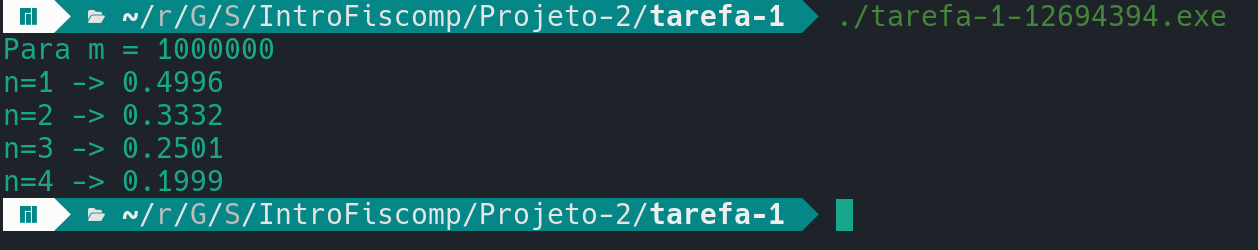
\includegraphics[width=14cm]{images/tarefa-1/imag1.png}
\caption*{Fonte: Compilado pelo Autor.}
\label{fig:tarefa 1 - código exibido na tela}
\end{figure}

\vspace*{2\baselineskip}

\begin{figure}[h!]
\centering
\caption{Valores de $\langle x^n \rangle$ para n entre 1 e 10}
  \centering
  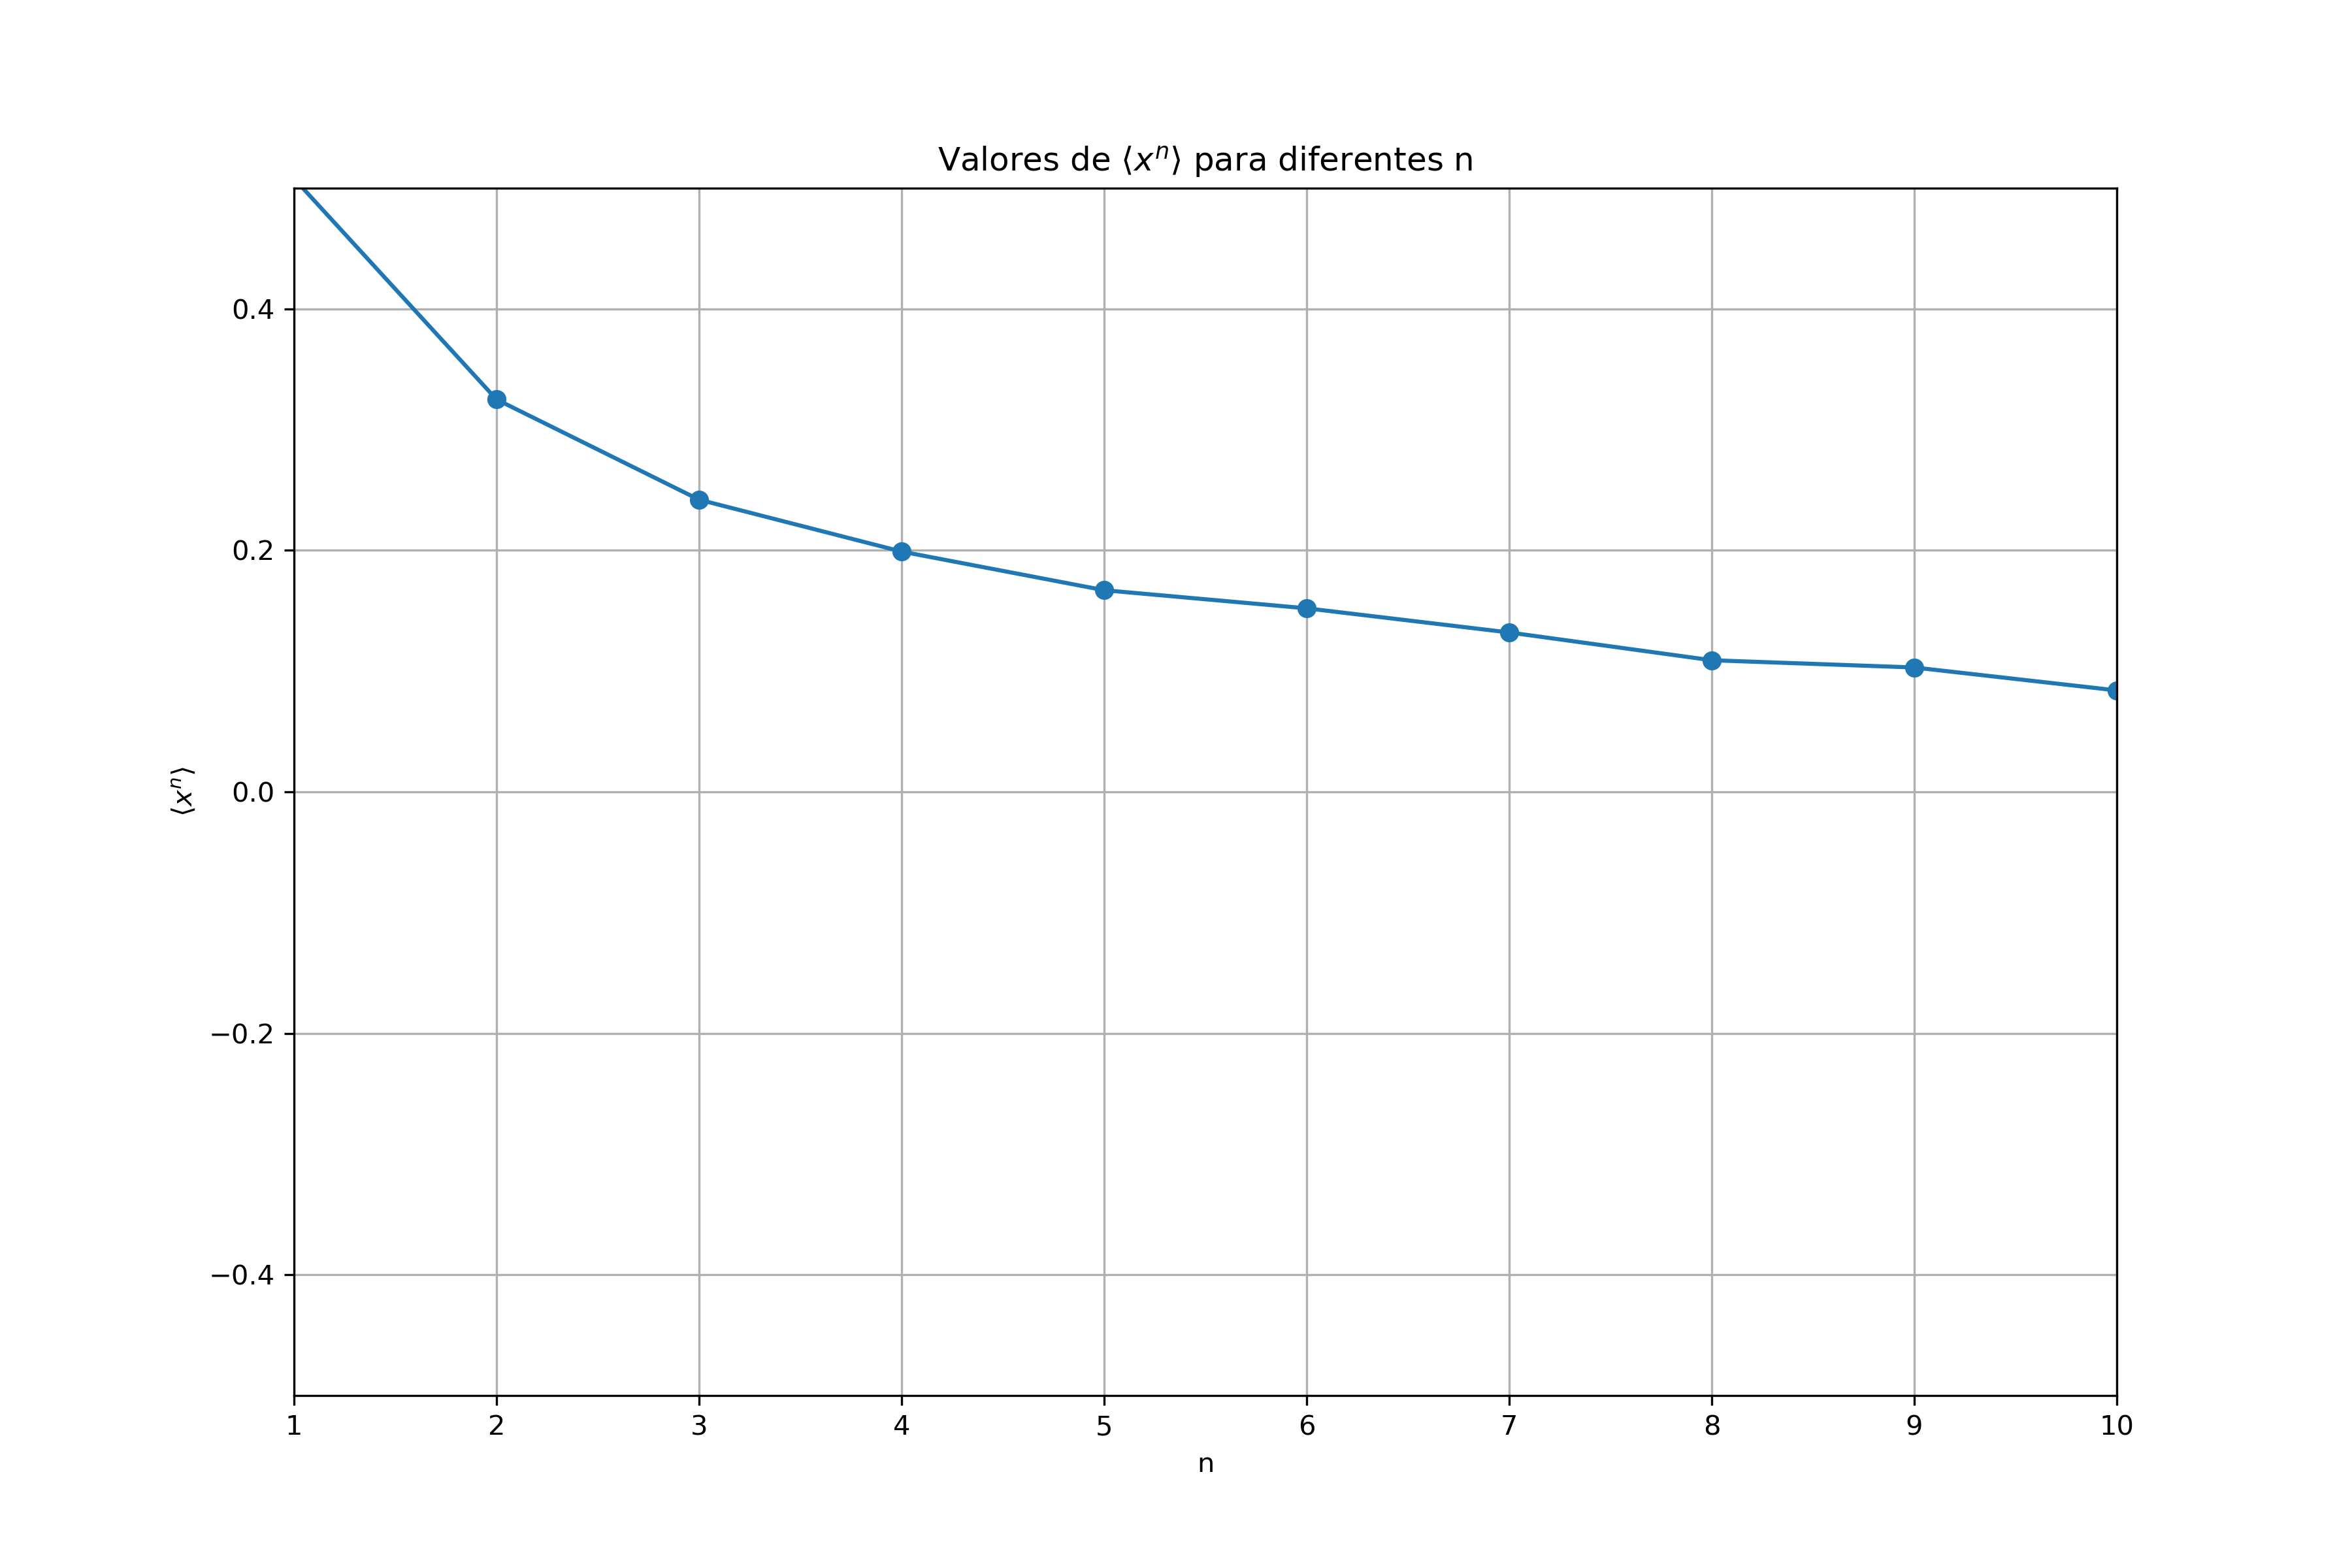
\includegraphics[width=14cm]{images/tarefa-1/fig_tarefa1_2.png}
\caption*{Fonte: Compilado pelo Autor.}
\label{fig:tarefa 1 - <x^n> para difererentes n =1,10}
\end{figure}

\vspace*{2\baselineskip}

\begin{figure}[h!]
\centering
\caption{Histograma que mostra a distribuição de valores para a função \textbf{rand()}, variando entre 0 e 1.}
  \centering
  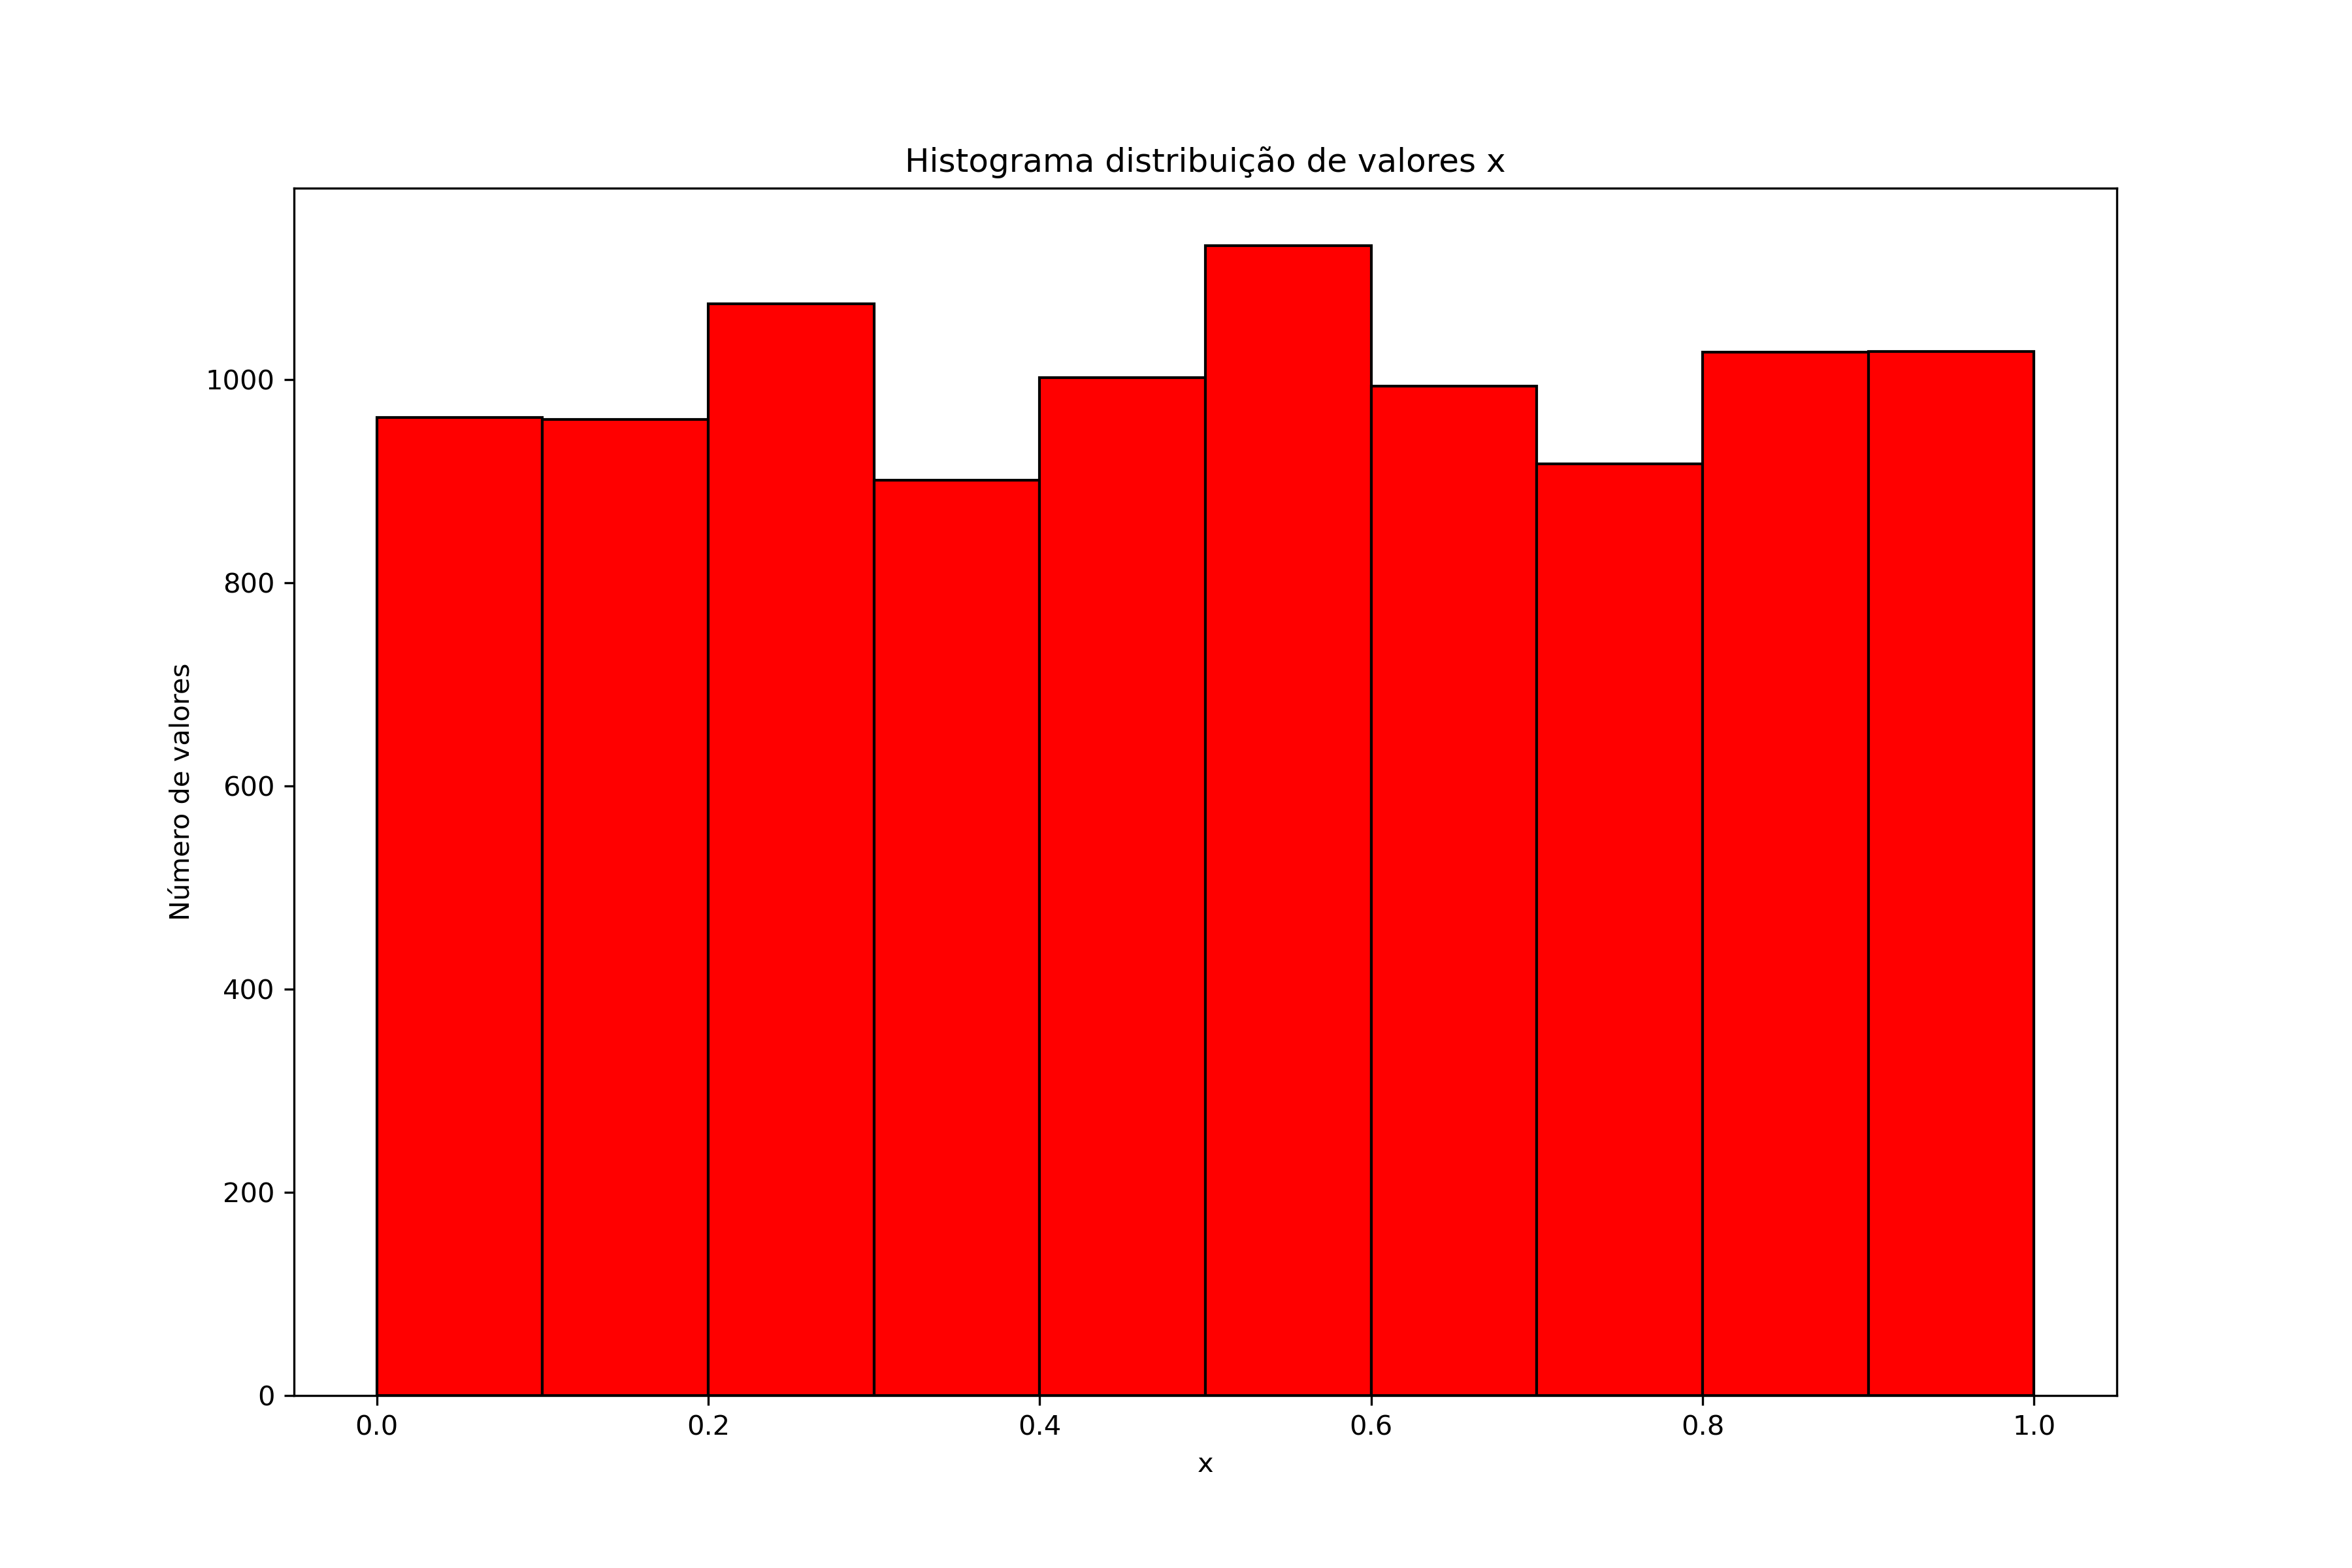
\includegraphics[width=14cm]{images/tarefa-1/fig_tarefa1_3.png}
\caption*{Fonte: Compilado pelo Autor.}
\label{fig:tarefa 1 - histograma rand()}
\end{figure}

\chapter*{Tarefa - 2}

\section*{Enunciado}

\begin{figure}[h!]
\centering
\caption{Enunciado da Tarefa 2.}
\centering
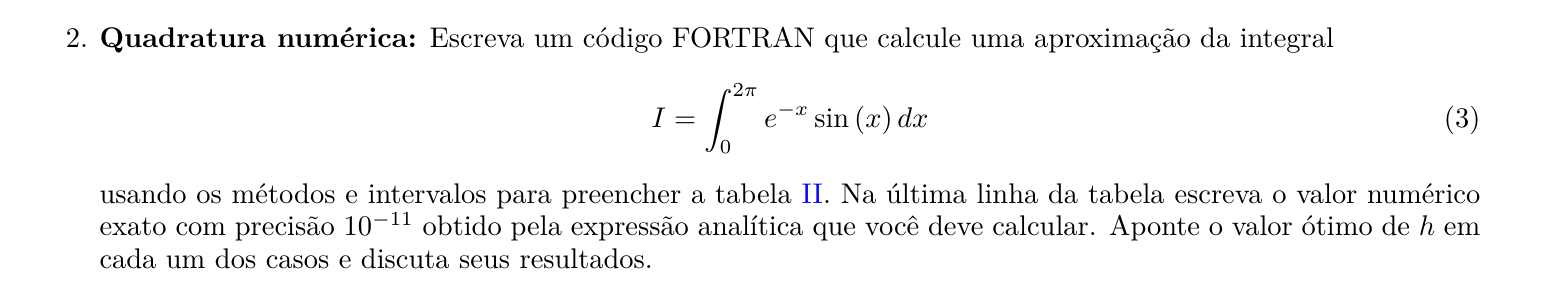
\includegraphics[width=16cm]{images/tarefa-2/enunciado-tarefa-2.png}
\caption*{Fonte: Compilado pelo Autor.}
\label{fig:tarefa 2 - Enunciado}
\end{figure}


\begin{figure}[h!]
\centering
\caption{Tarefa enunciado da Tarefa 2.}
\centering
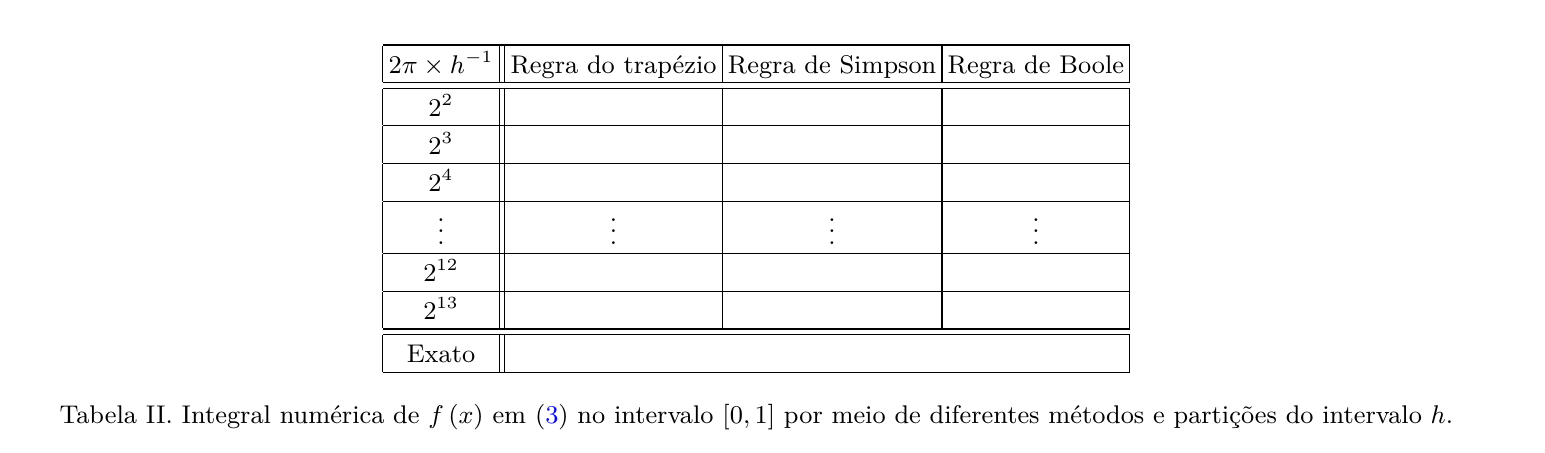
\includegraphics[width=17cm]{images/tarefa-2/tabela-enunciado-tarefa-2.png}
\caption*{Fonte: Compilado pelo Autor.}
\label{fig:tarefa 2 - Tabela Enunciado}
\end{figure}

\section*{Código}


\begin{figure}[H]
\centering
\caption{Função principal do código.}
\centering

\begin{lstlisting}
        program main
        implicit real*8 (a-h,o-z)

C       Constantes

        pi = acos(-1d0)

        a = 0d0
        b = 2d0*pi

C       Variáveis

        rval = 0.5d0*(1d0-exp(-2d0*pi))

        open(unit=1,file='saida-1-12694394.txt')

        do i = 2,13
        n = 2**i
        write(1,7) i,trap(a,b,n),simp(a,b,n),boole(a,b,n)
        end do
        write(1,3) rval
3       format(F16.11)
7       format(I3,3(',',F16.12))
        
        close(1)
        end program main
\end{lstlisting}

\caption*{Fonte: Compilado pelo Autor.}
\label{fig:tarefa 2 - função principal do código}
\end{figure}


\begin{figure}[H]
\centering
\caption{Função principal do código.}
\centering

\begin{lstlisting}
        function f(x)
        implicit real*8 (a-h,o-z)

        f = exp(-x)*sin(x)
        return
        end function f
\end{lstlisting}

\caption*{Fonte: Compilado pelo Autor.}
\label{fig:tarefa 2 - função estudada}
\end{figure}

\begin{figure}[H]
\centering
\caption{Função principal do código.}
\centering

\begin{lstlisting}
        function trap(a,b,n)
        implicit real*8 (a-h,o-z)

        h = (b-a)/n
        trap = 0d0
        do i = 1,n
            x = a + (i-1)*h
            rr = 0.5d0*h*(f(x+h)+f(x))
            trap = trap + rr
        end do

        return
        end function trap
\end{lstlisting}

\caption*{Fonte: Compilado pelo Autor.}
\label{fig:tarefa 2 - função trap}
\end{figure}

\begin{figure}[H]
\centering
\caption{Função principal do código.}
\centering

\begin{lstlisting}
        function boole(a,b,n)
        implicit real*8 (a-h,o-z)


        h = (b-a)/n
        boole = 0d0
        do i = 1,n
        x = a+(i-1)*h
        r1 = (2d0/45d0)*h
        r2 =(7d0*f(x-2d0*h)+7d0*f(x+2d0*h))
        r3 = (32d0*f(x-h)+12*f(x+h)+32d0*f(x+h))

        boole = boole + r1*(r2 + r3)/4d0
        end do

        return
        end function boole
\end{lstlisting}

\caption*{Fonte: Compilado pelo Autor.}
\label{fig:tarefa 2 - função boole}
\end{figure}

\begin{figure}[H]
\centering
\caption{Função principal do código.}
\centering

\begin{lstlisting}
        function simp(a,b,n)
        implicit real*8 (a-h,o-z)


        h = (b-a)/n
        simp = 0d0

        do i = 1,n
        x = a+(i-1)*h
        rr = (3d0*h/8d0)*(f(x)+3d0*f(x+h)+3d0*f(x+2d0*h)+f(x+3d0*h))
        simp = simp + rr/3d0
        end do

        return
        end function simp
\end{lstlisting}

\caption*{Fonte: Compilado pelo Autor.}
\label{fig:tarefa 2 - função simp}
\end{figure}


\section*{Descrição do código}
O programa \texttt{main} tem como objetivo calcular numericamente 
a integral da função

\begin{equation}
	I = \int_{0}^{2\pi}e^{-x} \sin(x)dx
\end{equation}

\noindent 
utilizando diferentes métodos de 
integração numérica: regra do trapézio, regra de Simpson 3/8 e regra de Boole.  
As aproximações são avaliadas para valores de $n = 2^i$, com 
$i = 2,3,\ldots,13$, permitindo analisar a convergência dos métodos 
à medida que o número de subdivisões aumenta.

\bigskip
No início do código, é utilizada a diretiva:

\vspace*{1\baselineskip}
\begin{lstlisting}
implicit real*8 (a-h,o-z)
\end{lstlisting}

\noindent
que define todas as variáveis cujos nomes começam com as letras 
de \textbf{a} a \textbf{h} e \textbf{o} a \textbf{z} como números reais 
de dupla precisão. Em seguida, o programa define constantes:

\vspace*{1\baselineskip}
\begin{lstlisting}
pi = acos(-1d0)
a = 0d0
b = 2d0*pi
\end{lstlisting}

\noindent
e o valor exato para a integral estudada:

\vspace*{1\baselineskip}
\begin{lstlisting}
rval = 0.5d0*(1d0-exp(-2d0*pi))
\end{lstlisting}

\noindent
O arquivo de saída é aberto com o comando:

\vspace*{1\baselineskip}
\begin{lstlisting}
open(unit=1,file='saida-1-12694394.txt')
\end{lstlisting}

\bigskip
No bloco principal, o programa entra em um laço:

\vspace*{1\baselineskip}
\begin{lstlisting}
do i = 2,13
    n = 2**i
    write(1,7) i,trap(a,b,n),simp(a,b,n),boole(a,b,n)
end do
\end{lstlisting}

\noindent
Em cada iteração, $n = 2^i$ define o número de subdivisões, e as funções 
\texttt{trap}, \texttt{simp} e \texttt{boole} calculam a integral usando 
as respectivas regras. Os resultados são escritos no arquivo de saída com o formato:

\vspace*{1\baselineskip}
\begin{lstlisting}
7 format(I3,3(',',F16.12))
\end{lstlisting}

\noindent
Após o laço, o valor de referência \texttt{rval} é escrito no arquivo com o formato:

\vspace*{1\baselineskip}
\begin{lstlisting}
3 format(F16.11)
\end{lstlisting}

\noindent
Por fim, o arquivo é fechado com:

\vspace*{1\baselineskip}
\begin{lstlisting}
close(1)
\end{lstlisting}

\subsection*{Funções auxiliares}

As funções implementam diferentes métodos de integração numérica sobre $[a,b]$.

\begin{enumerate}
    \item \textbf{Função \texttt{f(x)}} \\
    Define a função a ser integrada:
    \begin{equation}
        f(x) = e^{-x} \sin(x)
    \end{equation}

    \item \textbf{Função \texttt{trap(a,b,n)}} — Regra do Trapézio \\
    Aproxima a integral por:
    \begin{equation}
        \int_a^b f(x)\,dx \approx \sum_{i=1}^{n} \frac{h}{2}\Big(f(x_i)+f(x_{i+1})\Big),
    \end{equation}
    onde $h = (b-a)/n$ e $x_i = a + (i-1)h$.

    \item \textbf{Função \texttt{simp(a,b,n)}} — Regra de Simpson 3/8 \\
    Aproximação de quarta ordem que utiliza quatro pontos por subintervalo:
    \begin{equation}
        \int_{x_0}^{x_0+3h} f(x)\,dx \approx \sum_{i=1}^{n} \frac{3h}{8} \Big(f(x_i) + 3f(x_{i+1}) + 3f(x_{i+2}) + f(x_{i+3})\Big).
    \end{equation}

    \item \textbf{Função \texttt{boole(a,b,n)}} — Regra de Boole \\
    Fórmula de quinta ordem que utiliza cinco pontos igualmente espaçados:
    \begin{equation}
        \int_{x_0}^{x_0+4h} f(x)\,dx \approx \sum_{i=1}^{n} \frac{2h}{45} \Big( 7f(x_i) + 32f(x_{i+1}) + 12f(x_{i+2}) + 32f(x_{i+3}) + 7f(x_{i+4}) \Big).
    \end{equation}
\end{enumerate}

\noindent
Dessa forma, o programa permite calcular a integral de $f(x)$ sobre 
$[0,2\pi]$ usando diferentes métodos, comparando a precisão e convergência 
dos esquemas numéricos conforme aumenta o número de subdivisões.

\section*{Resultados}


\begin{table}[h!]
\centering
\caption{Raízes de $f(x)$ em (4) por meio de diferentes métodos e números de iterações.}
\label{table:tarefa-3-resultados}
\begin{NiceTabular}{c|cc|c|cc}[hvlines, columns-width=2.2cm]
\CodeBefore
    \rowcolor{cyan}{1}
    \rowcolors{2}{cyan!25}{cyan!15}
\Body
    \RowStyle[color=white, bold]{}
    Iteração $2^i$ & \multicolumn{2}{c|}{\textbf{Trapézio}} & \textbf{Simpson 3/8} & \multicolumn{2}{c}{\textbf{Boole}} \\
    2 & \multicolumn{2}{c|}{0.31242555} & 0.14946221 & \multicolumn{2}{c}{-2.98119765} \\
    3 & \multicolumn{2}{c|}{0.44884307} & 0.30210410 & \multicolumn{2}{c}{-0.39096151} \\
    4 & \multicolumn{2}{c|}{0.48630565} & 0.41986759 & \multicolumn{2}{c}{0.33488498} \\
    5 & \multicolumn{2}{c|}{0.49586365} & 0.47382433 & \multicolumn{2}{c}{0.46461834} \\
    6 & \multicolumn{2}{c|}{0.49826485} & 0.49194786 & \multicolumn{2}{c}{0.49118674} \\
    7 & \multicolumn{2}{c|}{0.49886587} & 0.49717723 & \multicolumn{2}{c}{0.49718160} \\
    8 & \multicolumn{2}{c|}{0.49901617} & 0.49857980 & \multicolumn{2}{c}{0.49860535} \\
    9 & \multicolumn{2}{c|}{0.49905375} & 0.49894285 & \multicolumn{2}{c}{0.49895230} \\
    10 & \multicolumn{2}{c|}{0.49906315} & 0.49903519 & \multicolumn{2}{c}{0.49903794} \\
    11 & \multicolumn{2}{c|}{0.49906550} & 0.49905848 & \multicolumn{2}{c}{0.49905921} \\
    12 & \multicolumn{2}{c|}{0.49906608} & 0.49906432 & \multicolumn{2}{c}{0.49906451} \\
    13 & \multicolumn{2}{c|}{0.49906623} & 0.49906579 & \multicolumn{2}{c}{0.49906584} \\
    \hline
    \textbf{Exato} & \multicolumn{5}{c}{0.49906627863} \\
\end{NiceTabular}

\caption*{Fonte: Compilado pelo Autor}
\end{table}

\begin{figure}[h!]
\centering
\caption{Dados salvos no arquivo de saida para a Tarefa - 2.}
\centering
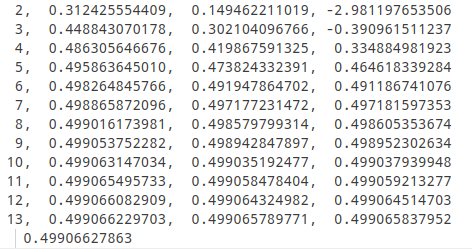
\includegraphics[width=16cm]{images/tarefa-2/tabela-1-tarefa-2.png}
\caption*{Fonte: Compilado pelo Autor.}
\label{fig:tarefa 2 - Tabela 1}
\end{figure}

\chapter*{Tarefa - 3}

\section*{Enunciado}

\begin{figure}[h!]
\centering
\caption{Enunciado da Tarefa 3.}
\centering
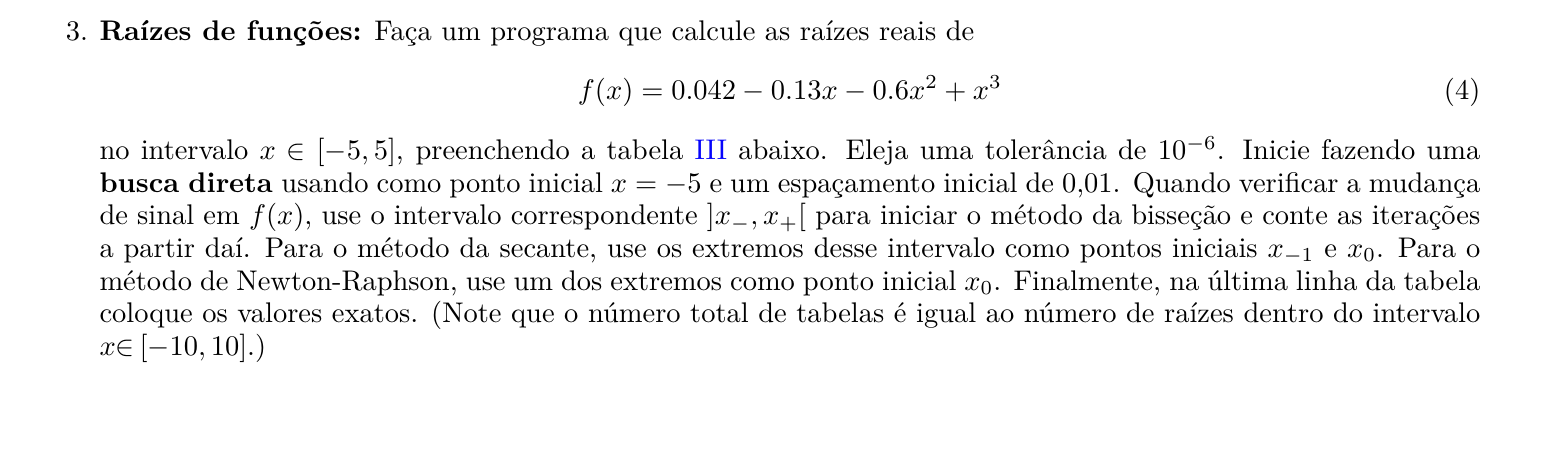
\includegraphics[width=16cm]{images/tarefa-3/enunciado-tarefa-3.png}
\caption*{Fonte: Compilado pelo Autor.}
\label{fig:tarefa 3 - Enunciado}
\end{figure}

\begin{figure}[h!]
\centering
\caption{Tarefa enunciado da Tarefa 3.}
\centering
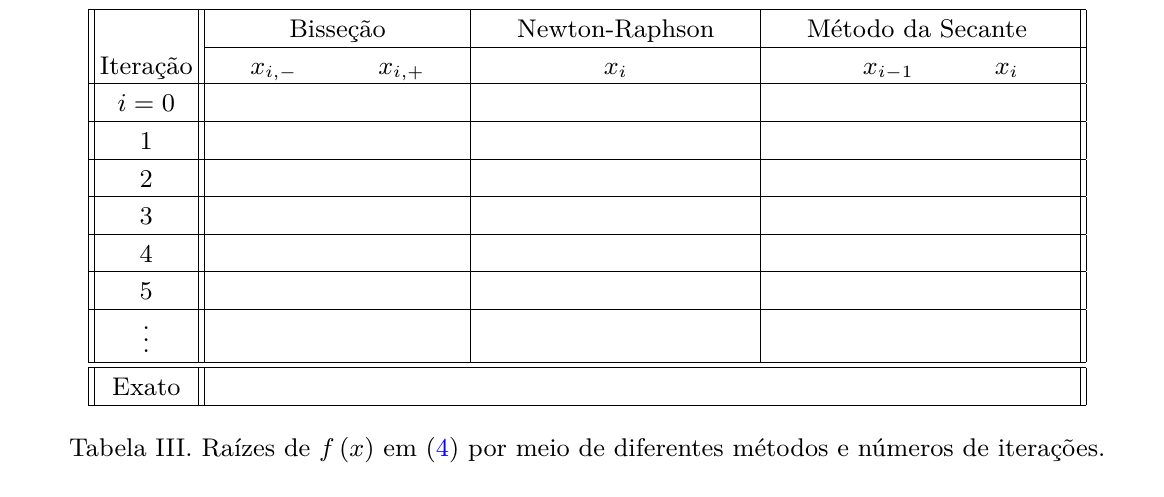
\includegraphics[width=16cm]{images/tarefa-3/tabela-enunciado-tarefa-3.png}
\caption*{Fonte: Compilado pelo Autor.}
\label{fig:tarefa 3 - Tabela Enunciado}
\end{figure}

\section*{Código}

\section*{Descrição do código}

O programa \texttt{main} tem como objetivo determinar numericamente as raízes da função

\begin{equation}
	f(x) = 0.042 - 0.13x - 0.6x^2 + x^3
\end{equation}

\noindent
utilizando três métodos iterativos de busca de raízes: 
\textbf{bisseção}, \textbf{Newton-Raphson} e \textbf{secante}.  
Cada método é implementado em uma função separada, e seus resultados são exibidos na tela e gravados em arquivos distintos.  
O código também avalia a convergência dos métodos a partir do número de iterações até atingir a tolerância estabelecida.

\bigskip
No início do programa, é utilizada a diretiva:

\vspace*{1\baselineskip}
\begin{lstlisting}
implicit real*8 (a-h,o-z)
\end{lstlisting}

\noindent
que define todas as variáveis cujos nomes começam com as letras 
de \textbf{a} a \textbf{h} e \textbf{o} a \textbf{z} como números reais 
de dupla precisão. Em seguida, são definidas as constantes principais:

\vspace*{1\baselineskip}
\begin{lstlisting}
a = 0.5d0
b = 5d0
tol = 1d-6
\end{lstlisting}

\noindent
onde $a$ e $b$ representam os limites iniciais do intervalo de busca e 
\texttt{tol} define a tolerância do erro desejado.

\bigskip
O programa principal chama as três funções numéricas responsáveis por 
calcular as raízes da função \texttt{f(x)}:

\vspace*{1\baselineskip}
\begin{lstlisting}
write(*,1) 'Bisseção: ', bissec(a,b,tol)
write(*,1) 'Newton-Raphson: ', raphson(a,tol)
write(*,1) 'Secante: ', secante(a,tol)
\end{lstlisting}

\noindent
Cada chamada executa o método correspondente e imprime o resultado com o formato:

\vspace*{1\baselineskip}
\begin{lstlisting}
1 format(A15,F14.12)
\end{lstlisting}

\noindent
permitindo visualizar o valor da raiz com 12 casas decimais de precisão.

\subsection*{Funções auxiliares}

As funções implementam tanto a função principal e sua derivada, 
quanto os três métodos iterativos de determinação de raízes.

\begin{enumerate}
	\item \textbf{Função \texttt{f(x)}} \\
	Define a função cúbica a ser analisada:
	\begin{equation}
		f(x) = 0.042 - 0.13x - 0.6x^2 + x^3
	\end{equation}

	\item \textbf{Função \texttt{df(x)}} \\
	Define a derivada de $f(x)$, necessária para o método de Newton-Raphson:
	\begin{equation}
		f'(x) = -0.13 - 1.2x + 3x^2
	\end{equation}

	\item \textbf{Função \texttt{bissec(a,b,tol)}} — Método da Bisseção \\
	O método da bisseção busca um intervalo $[a,b]$ onde há troca de sinal em $f(x)$.  
	Inicialmente, o código realiza uma varredura incremental com passo \texttt{stp = 0.01}, até encontrar um subintervalo onde $f(a)f(a+stp) < 0$.  
	Em seguida, aplica-se o procedimento iterativo:
	\begin{equation}
		c = \frac{a + b}{2}, \qquad
		\text{se } f(a)f(c) < 0, \; b = c, \; \text{senão } a = c
	\end{equation}
	até que $|b - a| < \texttt{tol}$.  
	Os valores intermediários de $c$ são gravados no arquivo:
	\vspace*{1\baselineskip}
	\begin{lstlisting}
	open(unit=13,file='saida-1-12694394.txt')
	\end{lstlisting}
	com o formato:
	\vspace*{1\baselineskip}
	\begin{lstlisting}
	14 format(I3,F16.12)
	\end{lstlisting}

	\item \textbf{Função \texttt{raphson(x,tol)}} — Método de Newton-Raphson \\
	Este método utiliza a fórmula iterativa:
	\begin{equation}
		x_{k+1} = x_k - \frac{f(x_k)}{f'(x_k)}
	\end{equation}
	As iterações continuam enquanto $|f(x)/f'(x)| > \texttt{tol}$.  
	A cada passo, o par $(\texttt{iter},x_k)$ é escrito no arquivo:
	\vspace*{1\baselineskip}
	\begin{lstlisting}
	open(unit=15,file='saida-2-12694394.txt')
	\end{lstlisting}
	usando o formato:
	\vspace*{1\baselineskip}
	\begin{lstlisting}
	16 format(I3,F16.12)
	\end{lstlisting}

	\item \textbf{Função \texttt{secante(x,tol)}} — Método da Secante \\
	Este método aproxima a derivada por diferenças finitas entre dois pontos consecutivos, conforme:
	\begin{equation}
		x_{k+1} = x_k - f(x_k)\frac{x_k - x_{k-1}}{f(x_k) - f(x_{k-1})}
	\end{equation}
	Sendo \texttt{stp = 0.01} o deslocamento inicial.  
	O processo é repetido até que $|x_{k+1} - x_k| < \texttt{tol}$.  
	Os valores iterativos são gravados em:
	\vspace*{1\baselineskip}
	\begin{lstlisting}
	open(unit=17,file='saida-3-12694394.txt')
	\end{lstlisting}
	com o formato:
	\vspace*{1\baselineskip}
	\begin{lstlisting}
	18 format(I3,F16.12)
	\end{lstlisting}
\end{enumerate}

\noindent
Assim, o programa permite determinar numericamente as raízes de uma função cúbica, 
comparando a eficiência e a convergência dos três métodos clássicos de busca de raízes: 
bisseção, Newton-Raphson e secante.  
Cada método gera um arquivo contendo as iterações realizadas, permitindo visualizar o comportamento da convergência.


\section*{Resultados}
As tabelas abaixo apresentam os resultados obtidos para as três raízes da função $f(x) = 0.042 - 0.13x - 0.6x^2 + x^3$ utilizando os métodos de Bissecção, Newton-Raphson e Secante.

\begin{table}[H]
\centering
\caption{Raízes de $f(x)$ por meio de diferentes métodos e números de iterações.}
\label{table:tarefa-3-resultados}
\begin{NiceTabular}{c|c|c|c}[hvlines, columns-width=2.8cm]
\CodeBefore
    \rowcolor{cyan}{1}
    \rowcolors{2}{cyan!25}{cyan!15}
\Body
    \RowStyle[color=white, bold]{}
    Iteração & \textbf{Bissecção} & \textbf{Newton} & \textbf{Secante} \\

    0  & -0.29500000 & -0.3000000 & -0.3000000 \\
    1  & -0.29750000 &            &      \\
    2  & -0.29875000 &            &      \\
    3  & -0.29937500 &            &      \\
    4  & -0.29968750 &            &      \\
    5  & -0.29984375 &            &      \\
    6  & -0.29992188 &            &      \\
    7  & -0.29996094 &            &      \\
    8  & -0.29998047 &            &      \\
    9  & -0.29999023 &            &      \\
    10 & -0.29999512 &            &      \\
    11 & -0.29999756 &            &      \\
    12 & -0.29999878 &            &      \\
    13 & -0.29999939 &            &      \\

    \hline
    \textbf{Raiz Aproximada} & \multicolumn{3}{c}{-0.3} \\
\end{NiceTabular}

\caption*{Fonte: Compilado pelo Autor.}
\end{table}

\begin{table}[H]
\centering
\caption{Raízes de $f(x)$ por meio de diferentes métodos e números de iterações.}
\label{table:tarefa-3-resultados-2}
\begin{NiceTabular}{c|c|c|c}[hvlines, columns-width=2.8cm]
\CodeBefore
    \rowcolor{cyan}{1}
    \rowcolors{2}{cyan!25}{cyan!15}
\Body
    \RowStyle[color=white, bold]{}
    Iteração & \textbf{Bissecção} & \textbf{Newton} & \textbf{Secante} \\

    0  & 0.1950000000& 0.19999938960& 0.200000000 \\
    1  & 0.1975000000&              &             \\
    2  & 0.1987500000&              &             \\
    3  & 0.1993750000&              &             \\
    4  & 0.1996875000&              &             \\
    5  & 0.1998437500&              &             \\
    6  & 0.1999218750&              &             \\
    7  & 0.1999609375&              &             \\
    8  & 0.1999804688&              &             \\
    9  & 0.1999902344&              &             \\
    10 & 0.1999951172&              &             \\
    11 & 0.1999975586&              &             \\
    12 & 0.1999987793&              &             \\
    13 & 0.1999993896&              &             \\

    \hline
    \textbf{Raiz Aproximada} & \multicolumn{3}{c}{0.2} \\
\end{NiceTabular}

\caption*{Fonte: Compilado pelo Autor.}
\end{table}

\begin{table}[H]
\centering
\caption{Raízes de $f(x)$ por meio de diferentes métodos e números de iterações.}
\label{table:tarefa-3-resultados-3}
\begin{NiceTabular}{c|c|c|c}[hvlines, columns-width=2.8cm]
\CodeBefore
    \rowcolor{cyan}{1}
    \rowcolors{2}{cyan!25}{cyan!15}
\Body
    \RowStyle[color=white, bold]{}
    Iteração & \textbf{Bissecção} & \textbf{Newton} & \textbf{Secante} \\

    0  & 0.695000000000 & 0.69999939 & 0.70000000 \\
    1  & 0.697500000000 &            &             \\
    2  & 0.698750000000 &            &             \\
    3  & 0.699375000000 &            &             \\
    4  & 0.699687500000 &            &             \\
    5  & 0.699843750000 &            &             \\
    6  & 0.699921875000 &            &             \\
    7  & 0.699960937500 &            &             \\
    8  & 0.699980468750 &            &             \\
    9  & 0.699990234375 &            &             \\
    10 & 0.699995117188 &            &             \\
    11 & 0.699997558594 &            &             \\
    12 & 0.699998779297 &            &             \\
    13 & 0.699999389648 &            &             \\

    \hline
    \textbf{Raiz Aproximada} & \multicolumn{3}{c}{0.7} \\
\end{NiceTabular}

\caption*{Fonte: Compilado pelo Autor.}
\end{table}

\begin{figure}[H]
\centering
\caption{Gráfico da função $f$.}
\centering
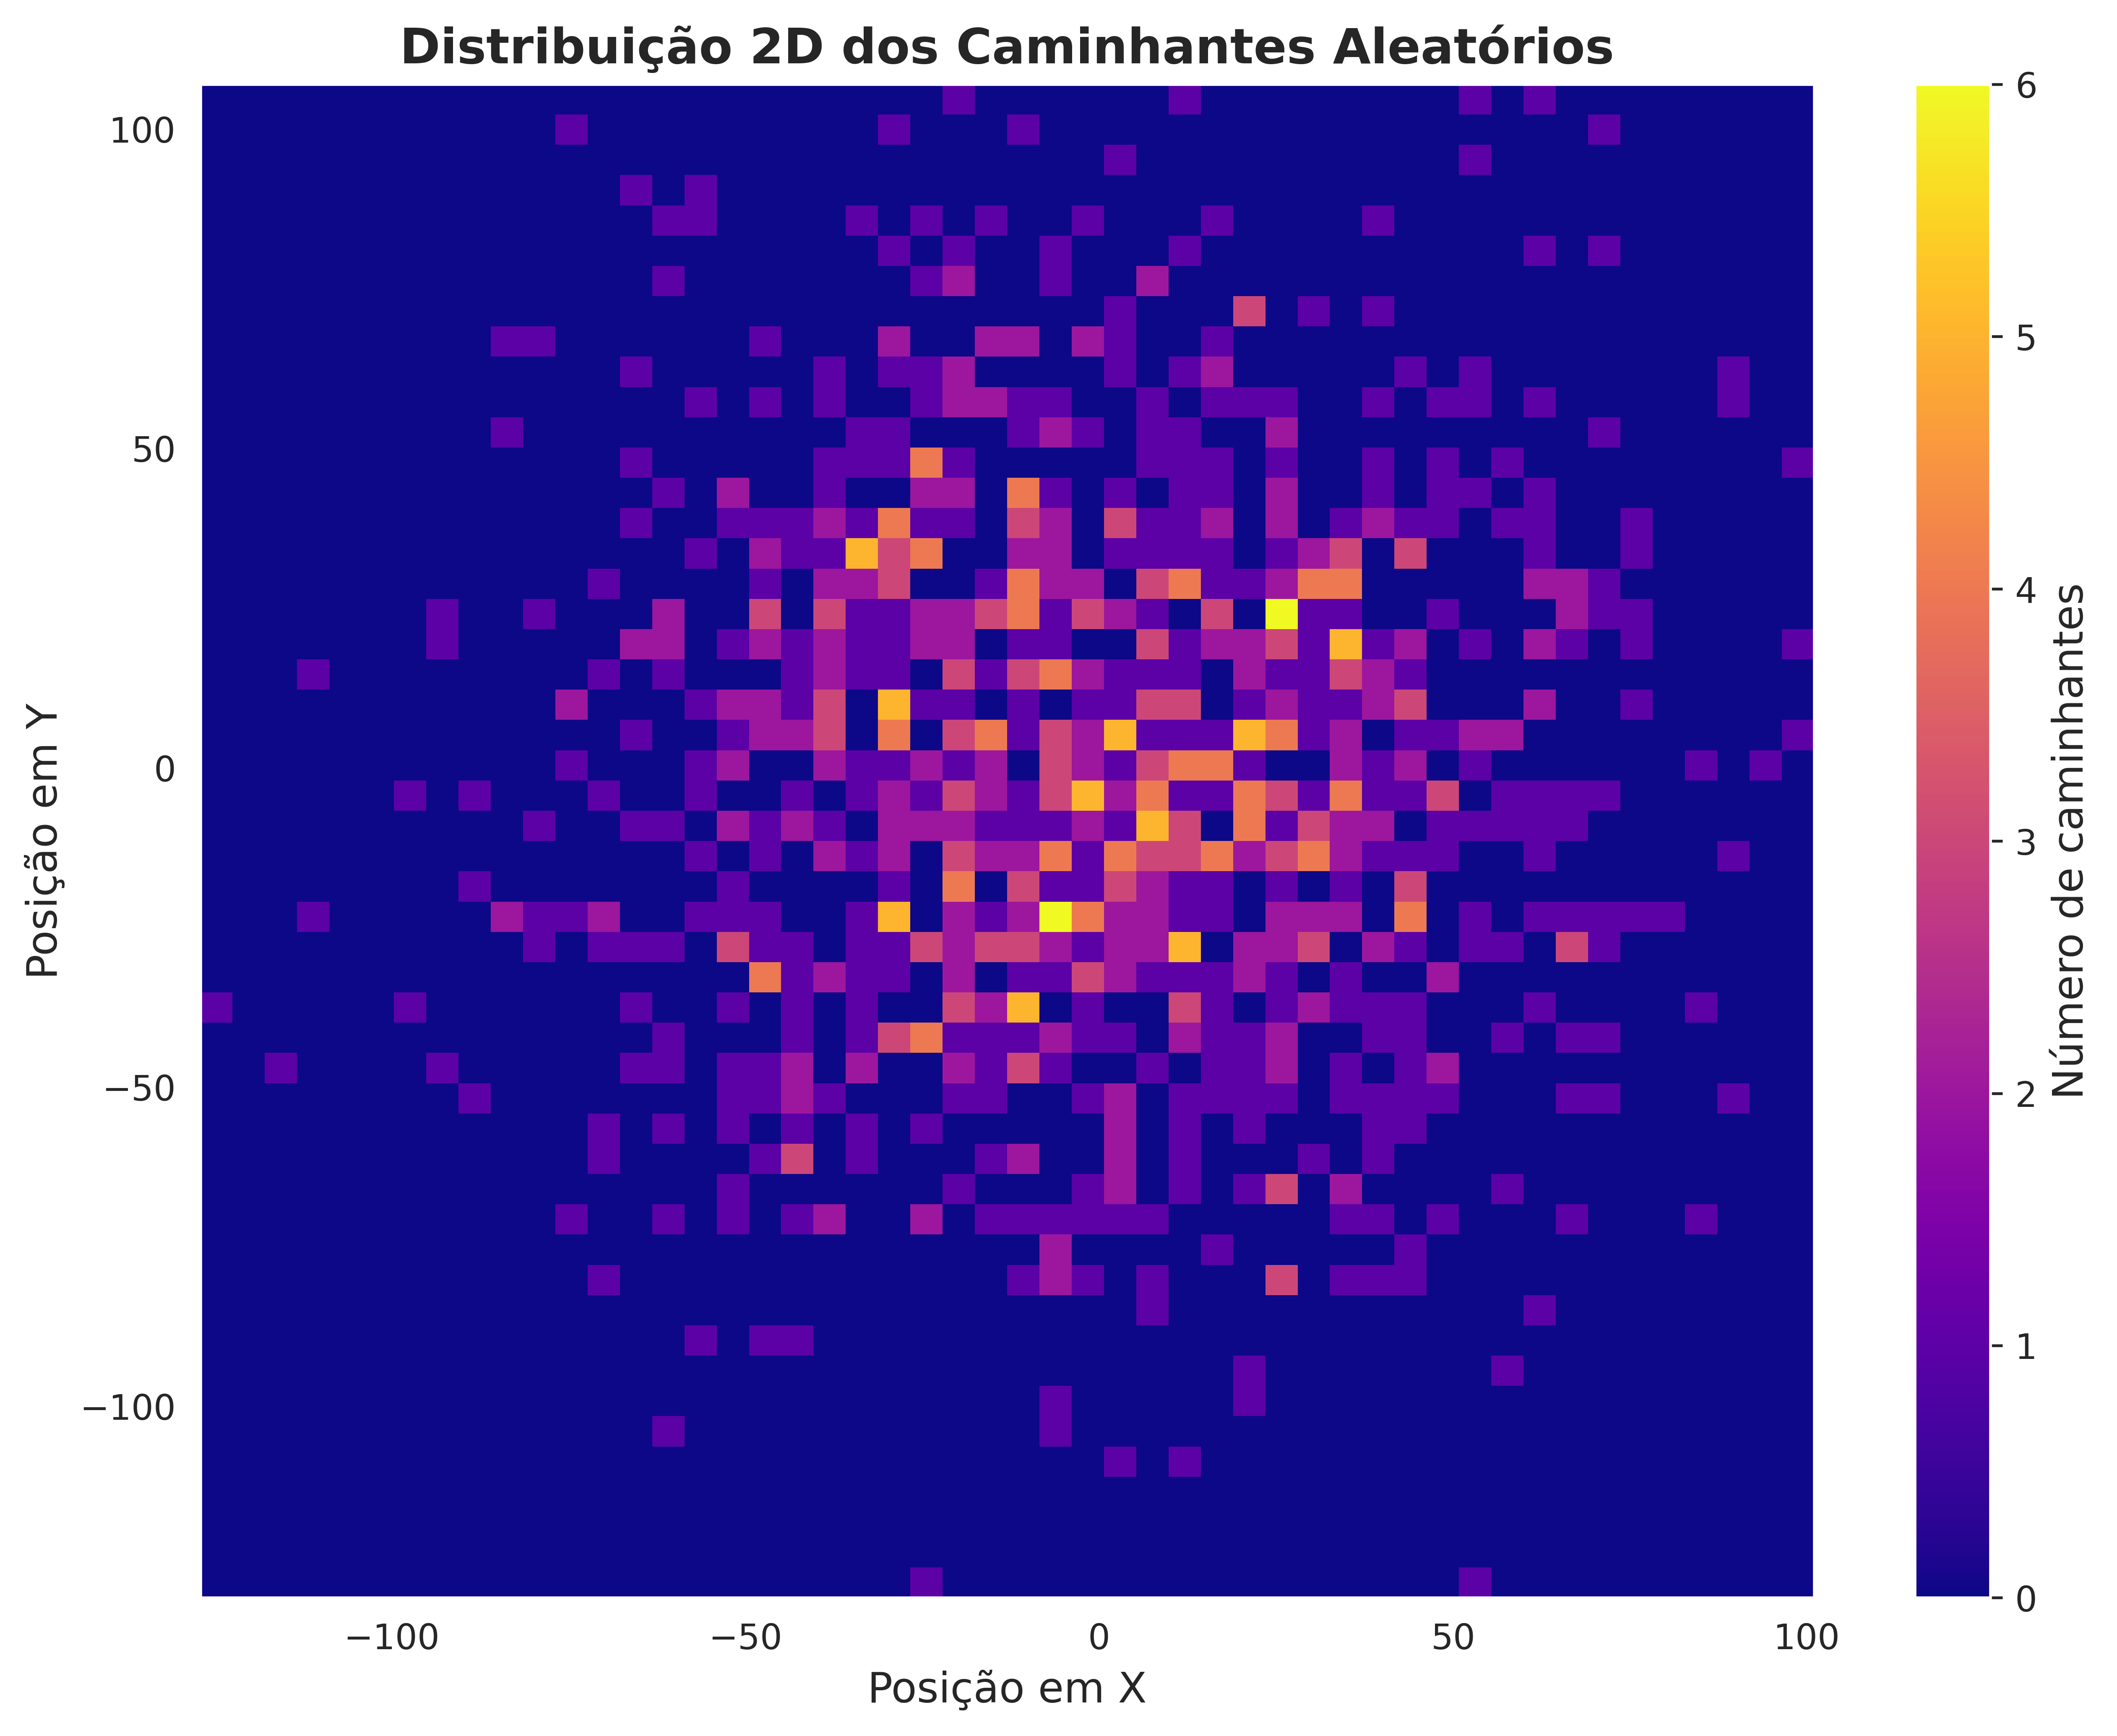
\includegraphics[width=16cm]{images/tarefa-3/tarefa-3-graf-1.png}
\caption*{Fonte: Compilado pelo Autor.}
\label{fig:tarefa 3 - Gráfico 1}
\end{figure}

\begin{figure}[H]
\centering
\caption{Gráfico da função $f$.}
\centering
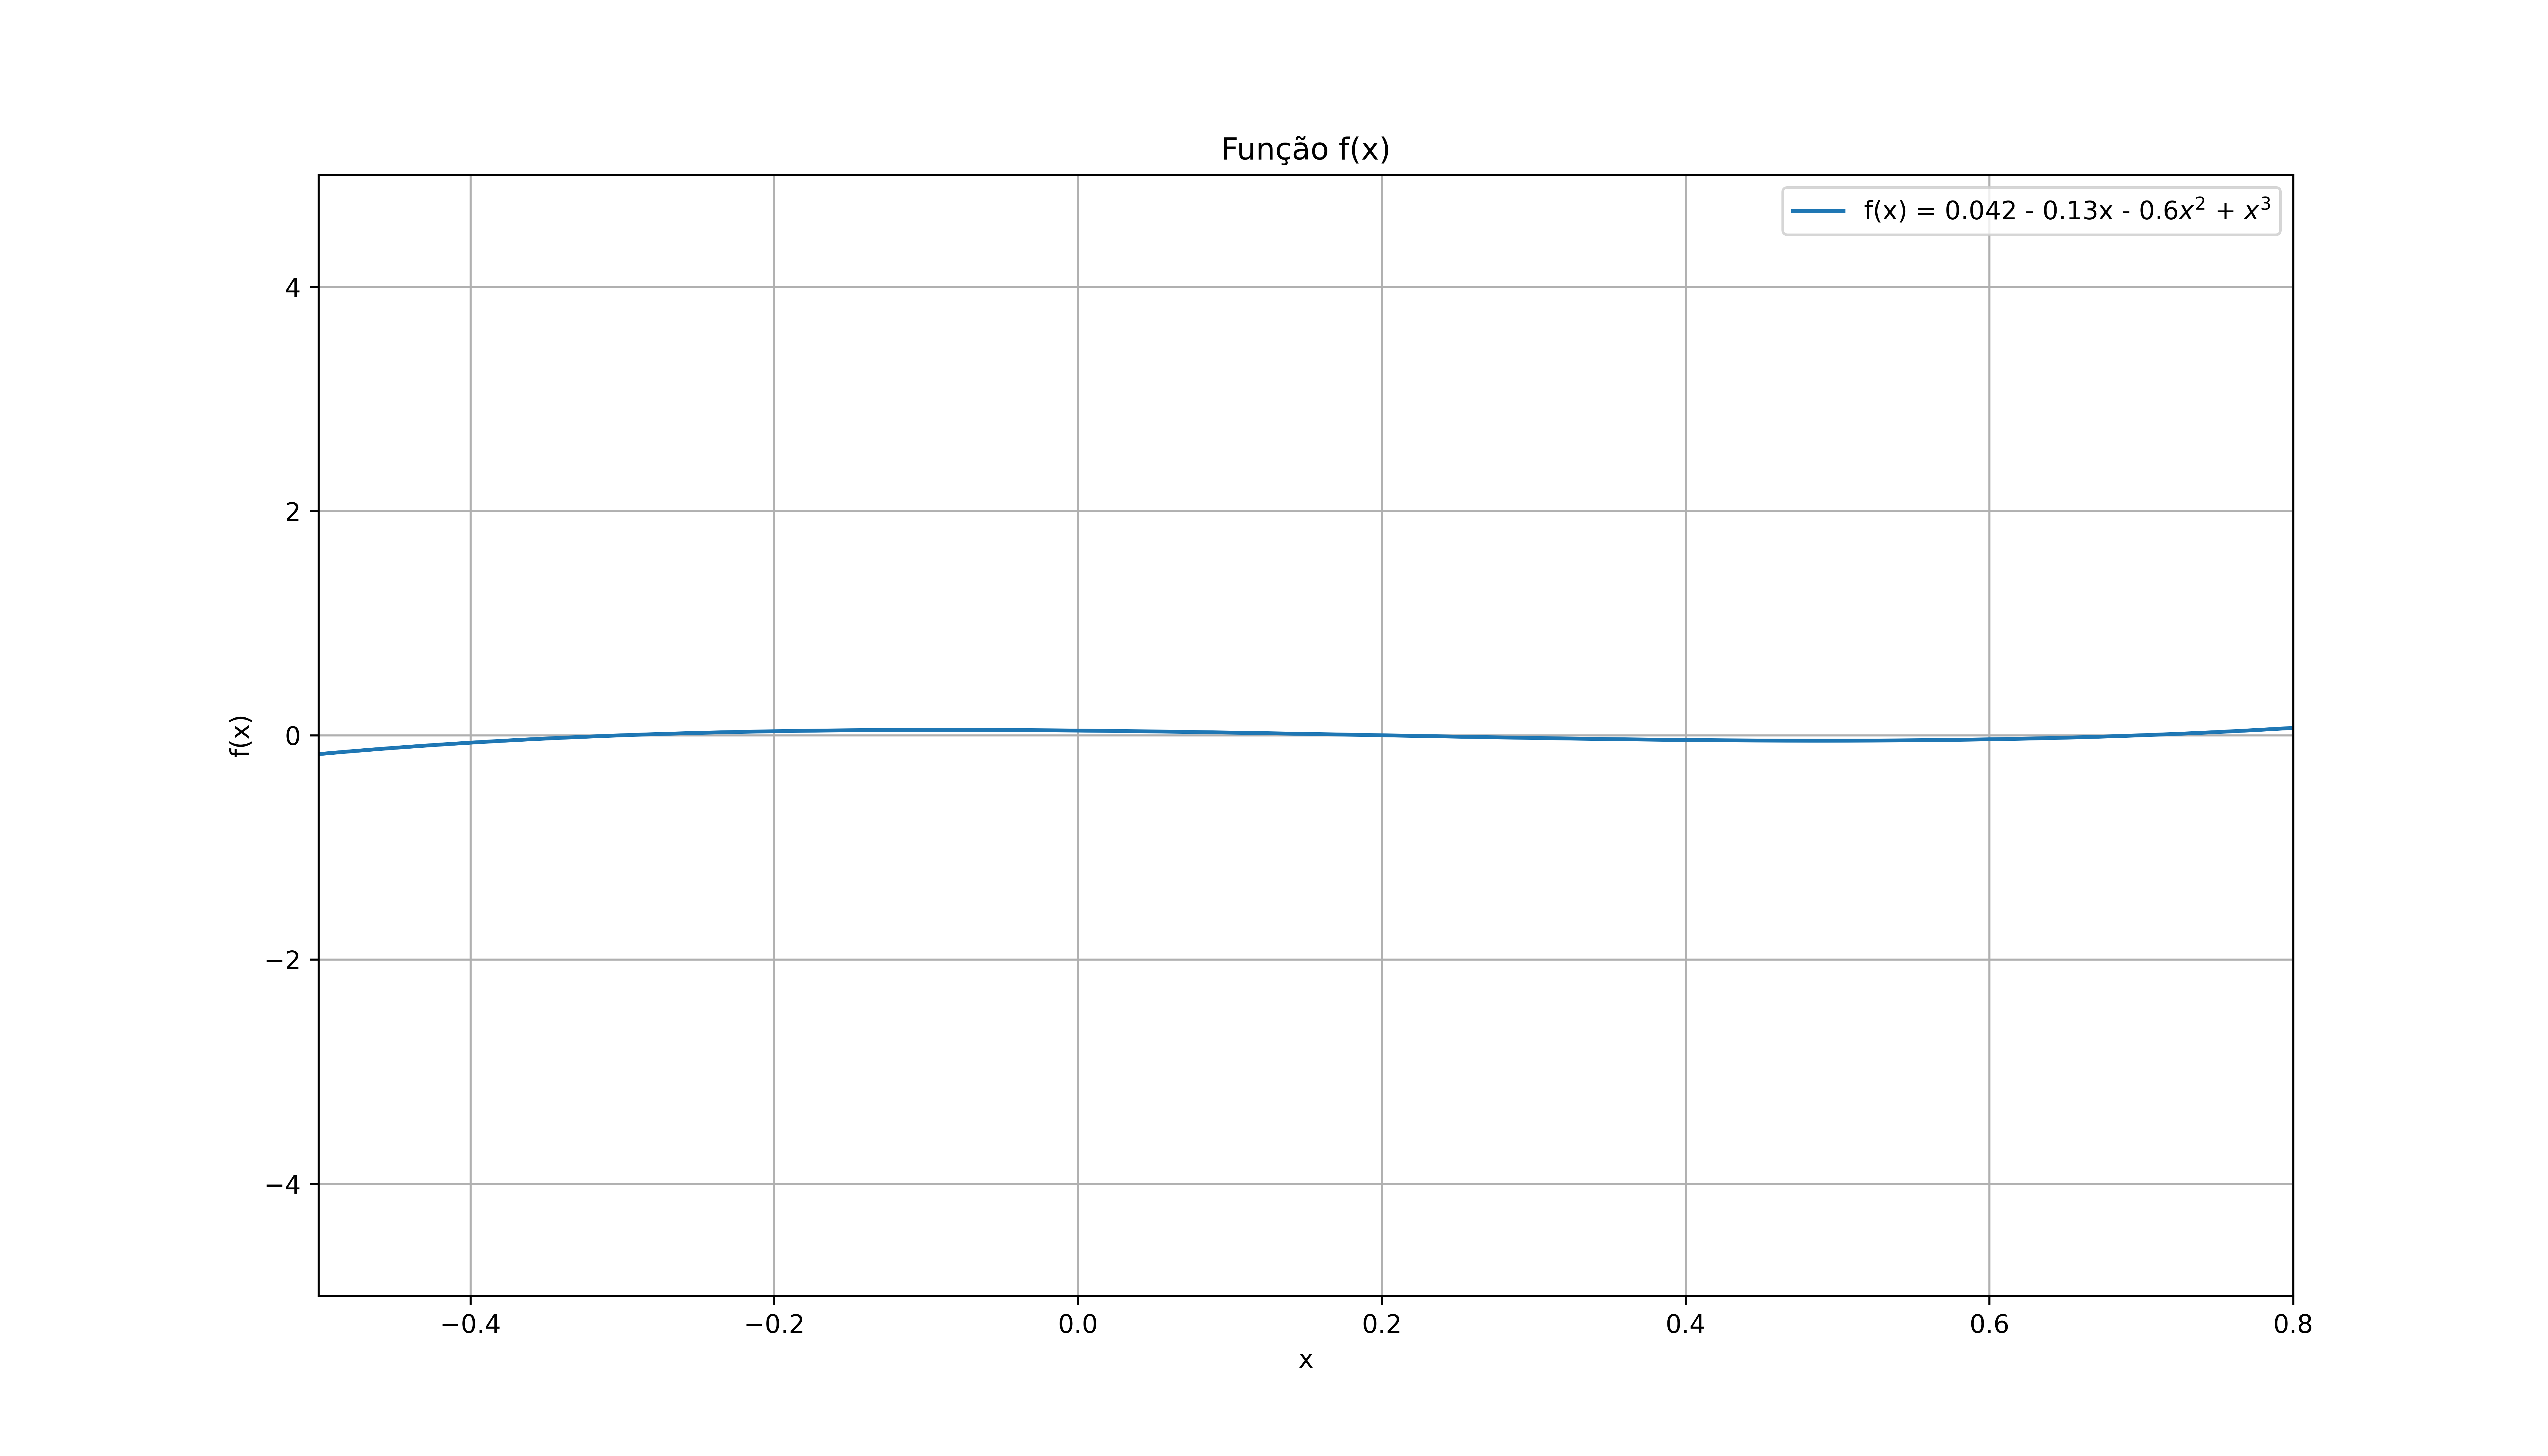
\includegraphics[width=16cm]{images/tarefa-3/tarefa-3-graf-2.png}
\caption*{Fonte: Compilado pelo Autor.}
\label{fig:tarefa 3 - Gráfico 2}
\end{figure}

\begin{figure}[H]
\centering
\caption{Gráfico da função $f$.}
\centering
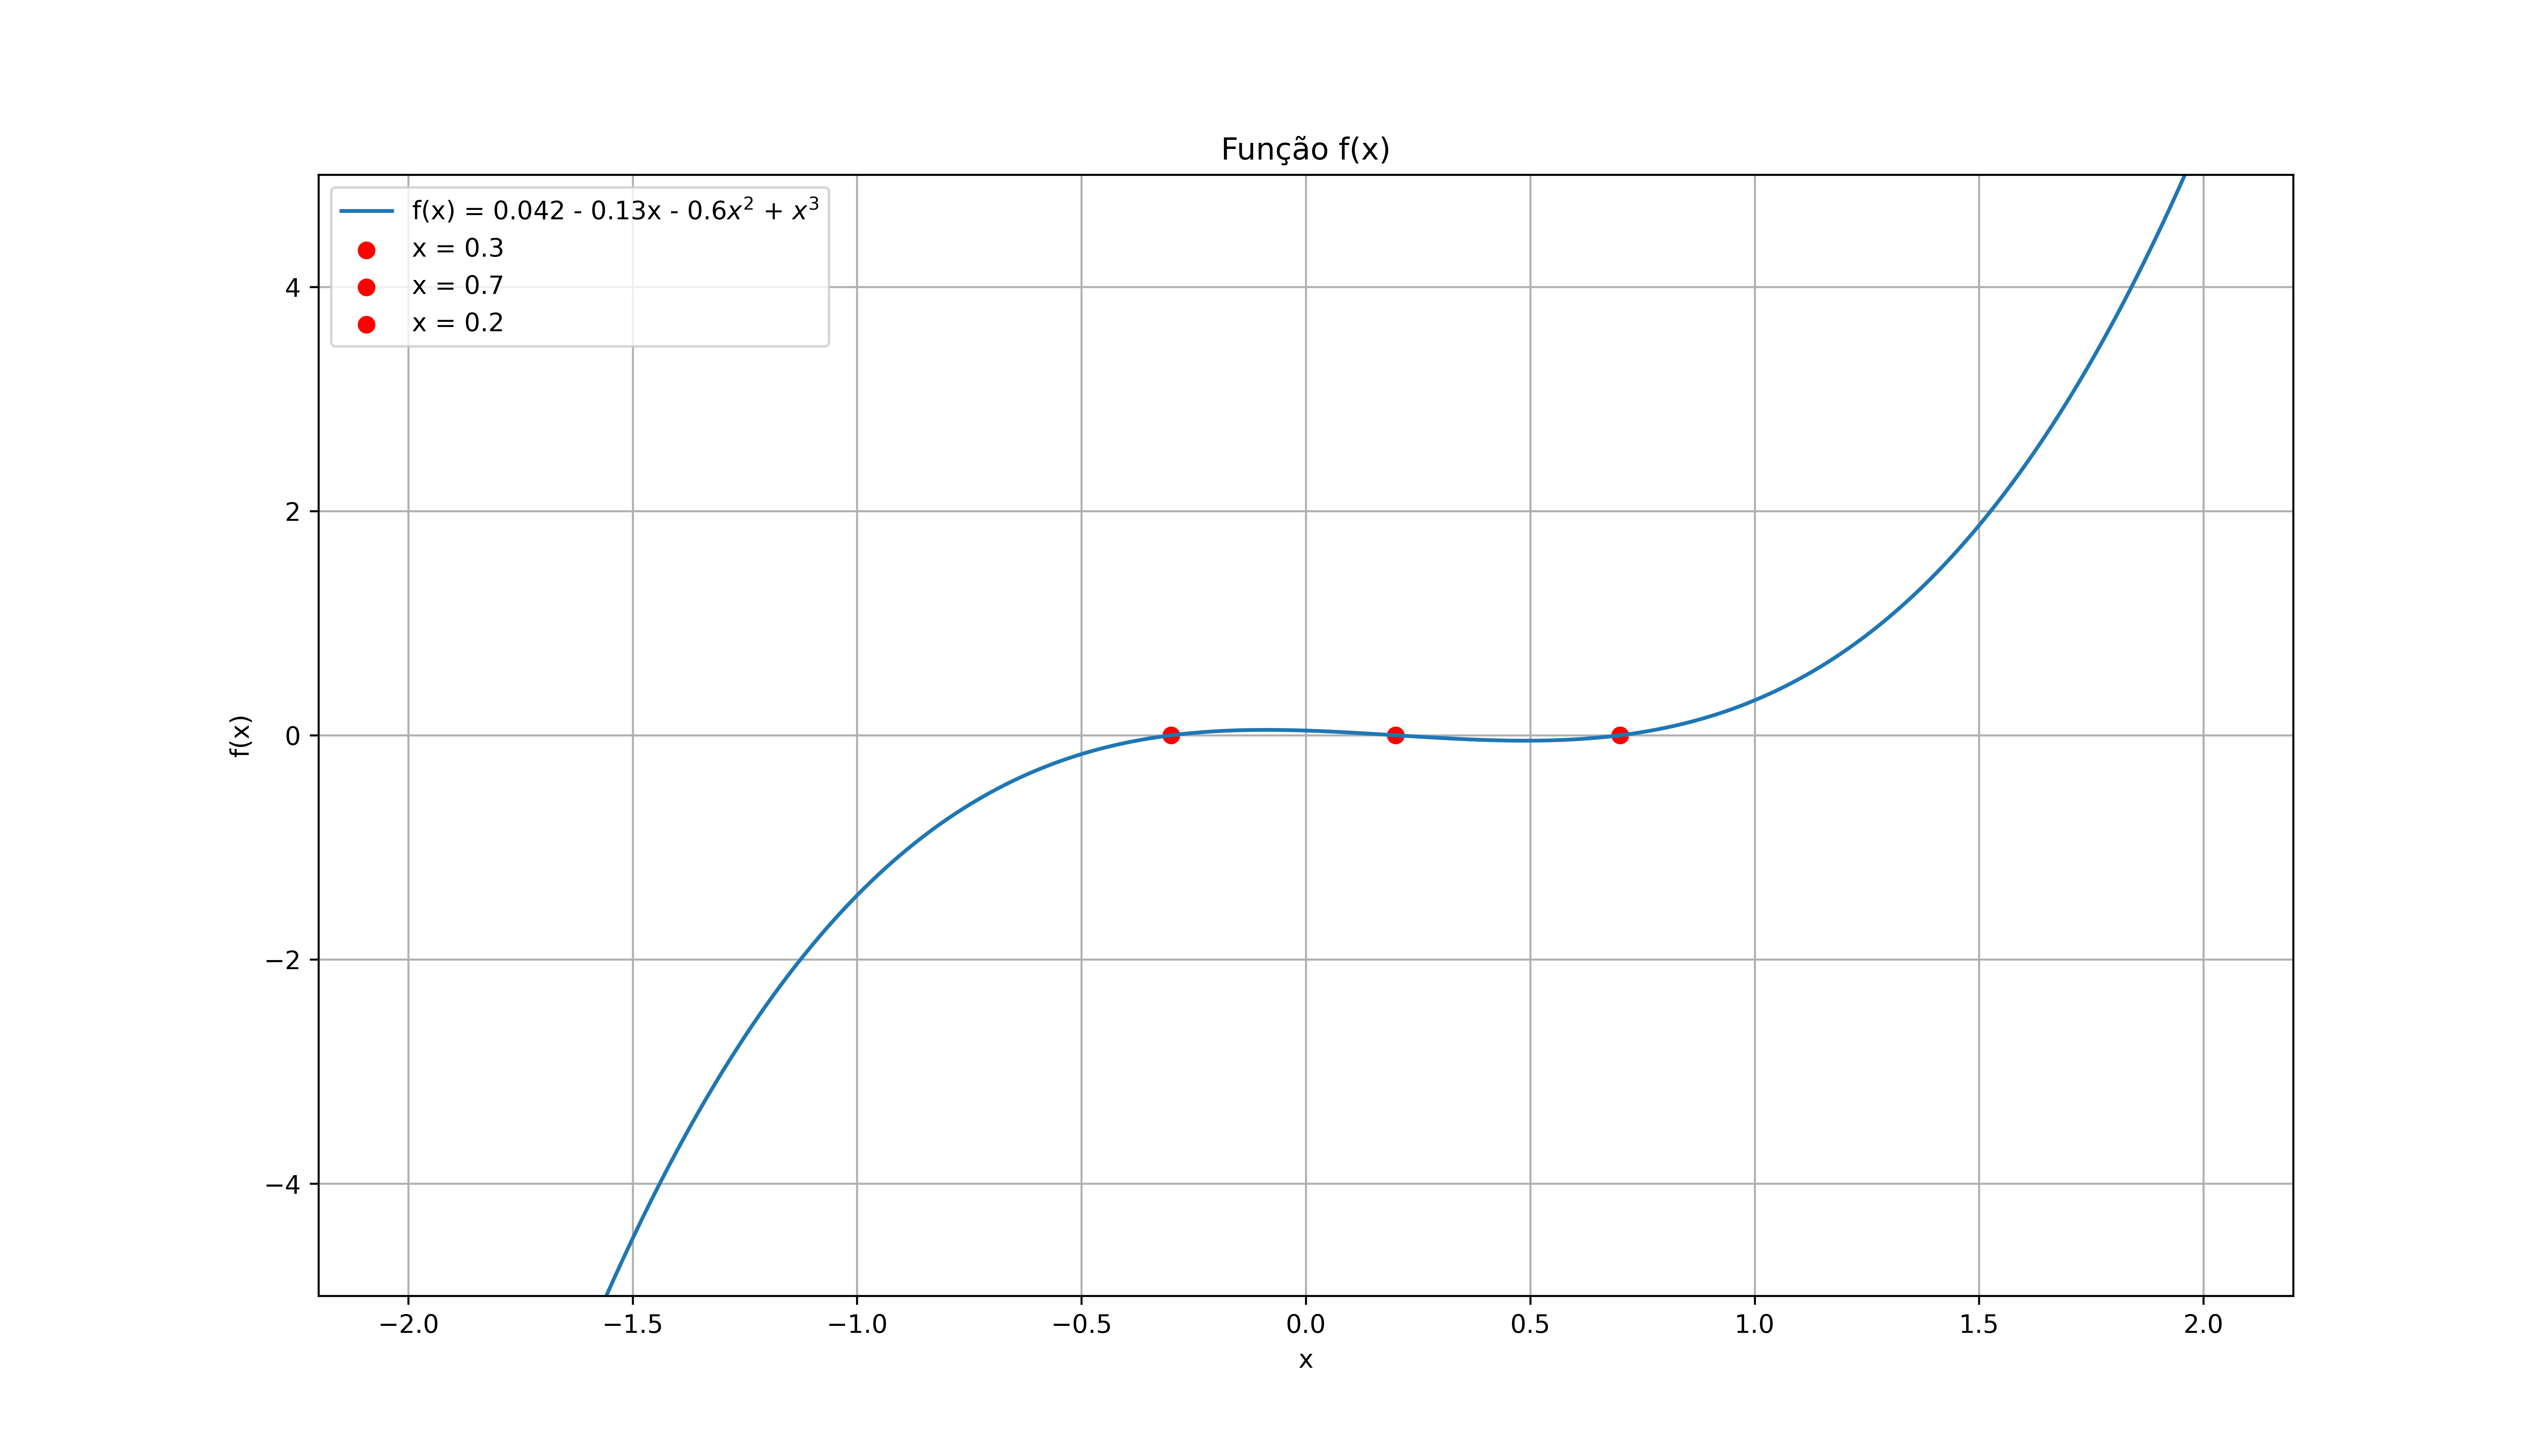
\includegraphics[width=16cm]{images/tarefa-3/tarefa-3-graf-3.png}
\caption*{Fonte: Compilado pelo Autor.}
\label{fig:tarefa 3 - Gráfico 3}
\end{figure}

\begin{figure}[H]
\centering
\caption{Gráfico da função $f$.}
\centering
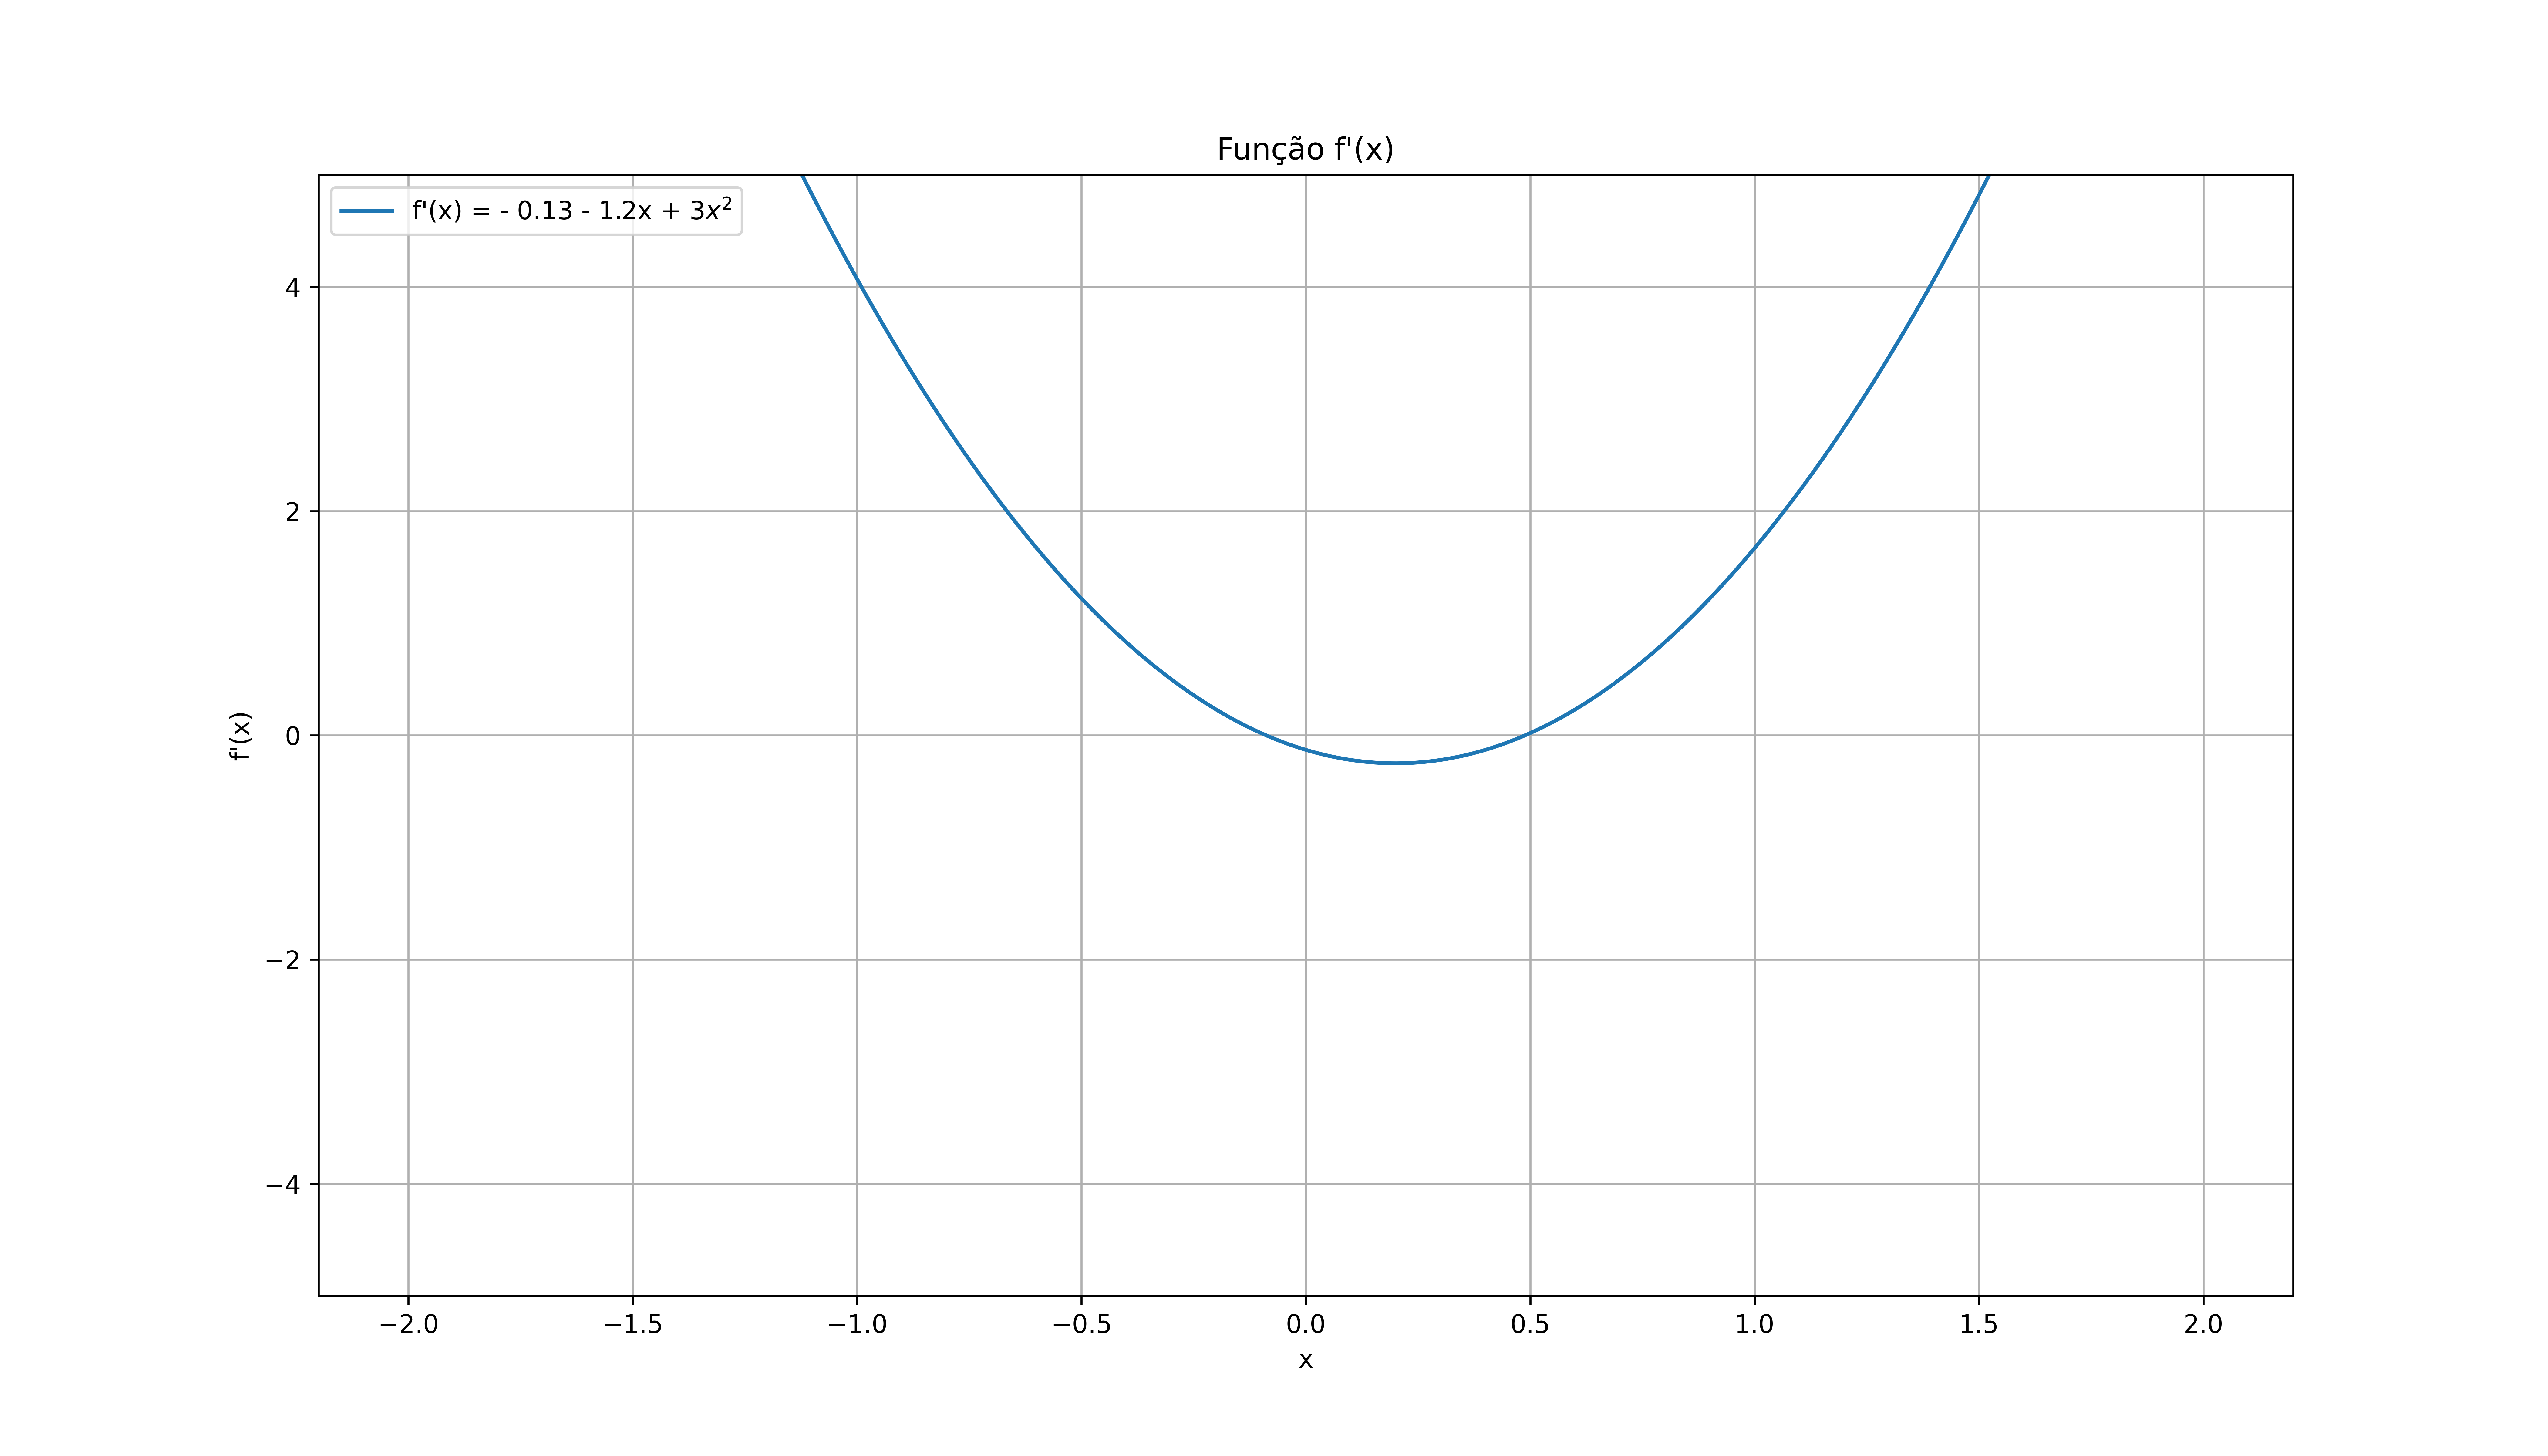
\includegraphics[width=16cm]{images/tarefa-3/tarefa-3-graf-4.png}
\caption*{Fonte: Compilado pelo Autor.}
\label{fig:tarefa 3 - Gráfico 4}
\end{figure}

\noindent
Ademais, é visto nos terminais os seguintes valores.

\begin{figure}[H]
\centering
\caption{Terminal a=-5.}
\centering
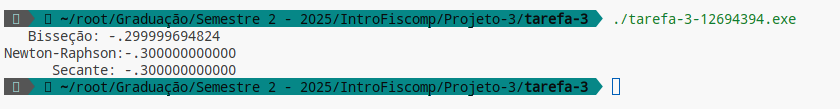
\includegraphics[width=16cm]{images/tarefa-3/tarefa-3-terminal-1.png}
\caption*{Fonte: Compilado pelo Autor.}
\label{fig:tarefa 3 - Terminal 1}
\end{figure}

\begin{figure}[H]
\centering
\caption{Terminal a=0.}
\centering
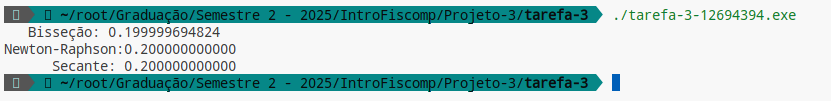
\includegraphics[width=16cm]{images/tarefa-3/tarefa-3-terminal-2.png}
\caption*{Fonte: Compilado pelo Autor.}
\label{fig:tarefa 3 - Terminal 2}
\end{figure}

\begin{figure}[H]
\centering
\caption{Terminal a=0.50.}
\centering
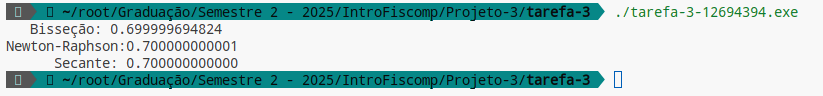
\includegraphics[width=16cm]{images/tarefa-3/tarefa-3-terminal-3.png}
\caption*{Fonte: Compilado pelo Autor.}
\label{fig:tarefa 3 - Terminal 3}
\end{figure}

\chapter*{Questão 4}

\section*{Enunciado}

\noindent
4. Vamos verificar o aumento da entropia e a flecha do tempo no exercício anterior. 
Calcule a entropia como função do número de passos $N$ das moléculas (que é proporcional 
ao tempo $t = N \Delta t$, onde $\Delta t$ é o intervalo de tempo médio entre passos). A entropia é dada por

\begin{equation}
S = - \sum_i P_i \ln P_i,
\end{equation}

\noindent
onde $P_i$ é a probabilidade de se encontrar o sistema em um certo micro-estado $i$. 
Para se definir o micro-estado $i$, definimos um reticulado (muito maior que o tamanho 
de um passo) e verificamos quantas moléculas encontramos em cada célula do reticulado.


\section*{Metodologia}

Nessa simulação é pedido para calcular o valor da entropia de um sistema com \textit{M} 
moléculas, realizando \textit{N} passos. 

Tendo em vista que a entropia do sistema cresce em função do tempo, este que é proporcional 
ao número de passos, $t = N(t-t_0)$, é possível simular o aumento de entropia utilizando 
um aumento no número de passos dados pelas moléculas.

\begin{equation} \label{entropia}
    S = -\sum_{i} P_i \ln{P_i}
\end{equation}

Tendo em vista que a entropia de um sistema é dada pela Equação \ref{entropia}, 
onde $P_i$ é a probabilidade de encontrar o sistema em um certo micro-estado, 
tal que o micro-estado é definido como sendo um reticulado de tamanho fixo 
no qual é medido o número de moléculas que lá estão.

\begin{equation} \label{micro-estado}
    P_i = \frac{K_i}{M}
\end{equation}

Desse modo, através da Equação \ref{micro-estado}, onde $K_i$ é o número de partículas 
no reticulado e $M$ é o número total de moléculas, é possível encontrar a probabilidade 
$P_i$ daquele micro-estado ocorrer.



\section*{Código}

A estrutura principal do código abre um arquivo de saída, percorre 
diferentes valores de $N$ (número de passos) e, para cada caso, chama a função \texttt{calc}, 
que realiza os cálculos necessários para estimar a entropia do sistema.

A função \texttt{calc} é o núcleo do programa. Inicialmente, é definido o tamanho do 
reticulado em função de $N$, bem como os micro-estados disponíveis. Em seguida, o reticulado 
é zerado, e os possíveis passos são definidos como deslocamentos de $\pm 1$ em cada direção. 

A simulação é então realizada para $m$ moléculas, que partem da origem e percorrem $N$ 
passos aleatórios. A cada passo, a direção é escolhida de forma estocástica, com igual 
probabilidade de caminhar no eixo $x$ ou no eixo $y$, e o reticulado registra a posição 
final das partículas.

Após a simulação, a função procede ao cálculo da entropia. O espaço é dividido em regiões 
do reticulado (as células), e conta-se o número de partículas em cada uma. A probabilidade 
$P_i$ de encontrar uma partícula em um micro-estado $i$ é obtida pela razão entre a ocupação 
da célula e o número total de partículas, normalizado pelo fator de discretização. 

Com esses valores, a função aplica a fórmula
\[
S = - \sum_i P_i \ln P_i,
\]
acumulando a contribuição de cada célula do reticulado. 

O valor de entropia calculado é então retornado para o programa principal, que o registra 
no arquivo de saída junto com o respectivo número de passos.


\begin{figure}[h!]
\centering
\caption{Função principal do código.}
\centering
\begin{lstlisting}
program main
        m = 1000
        open(unit=1,file='saida-1-12694394.txt')
        do i = 100,1000
                write(1,7) i,calc(m,i)
        end do
7               format(I12,',',F12.4)
        close(1)
end program main

\end{lstlisting}
\caption*{Fonte: Compilado pelo Autor.}
\label{fig:tarefa 4 - função principal do código}
\end{figure}

\begin{figure}[h!]
\centering
\caption{Função que realiza os cálculos.}
\centering
\begin{lstlisting}
function calc(m,n)
        parameter(iseed=1154)
        dimension ipos(-n:n,-n:n),istep(0:1)
        
        ! Número de micro estados
        irazao = n*0.1
        ! Tamanho do reticulado
        ksize = n/irazao 

        ! Da o seed para o rand()
        rr = rand(iseed)
        ! Inicia o vetor posição
        do i =-n,n
                do j = -n,n
                        ipos(i,j) = 0
                end do
        end do
        
        ! Valores dos passos
        istep(0) = 1
        istep(1) = -1
        

\end{lstlisting}

\caption*{Fonte: Compilado pelo Autor.}
\label{fig:tarefa 4 - função que realiza os cálculos}
\end{figure}




\begin{figure}[h!]
\centering
\caption{Função que realiza os cálculos.}
\centering
\begin{lstlisting}

        ! Realiza os cálculos
        do i = 1,m
                ix = 0
                iy = 0
                do j = 1,n
                idir = 2e0*rand()
                irand = 2e0*rand()

                if (idir .EQ. 0) then
                        ix = ix + istep(irand)
                else
                        iy = iy + istep(irand)
                endif
                end do
                ipos(ix,iy) = ipos(ix,iy) + 1
        end do
        
        ! Calculo reticulado
        calc = 0
        n1 = -n
        n2 = n1 + ksize
        do k =1,2*irazao
                rpro= 0e0

                do i = n1,n2
                        do j = n1,n2
                                rpro = rpro + ipos(i,j) 
                        end do
                end do
                
                rpro = rpro/(irazao)
                
                if (rpro .NE. 0e0) then
                        calc = calc - rpro*log(rpro)

                end if
                ! Muda o valor dos indices
                n1 = n2
                n2 = n2 + ksize
        end do
        return
end function calc
\end{lstlisting}

\caption*{Fonte: Compilado pelo Autor.}
\label{fig:tarefa 4 - função que realiza os cálculos}
\end{figure}

\newpage
\section*{Função calc}


A função calc(m,n) tem por objetivo simular $m$ trajetórias (ou “moléculas”) realizando $n$ passos
cada, registrar a posição final de cada trajetória em um reticulado discreto e, a partir da distribuição
espacial resultante, calcular uma aproximação da entropia de Shannon das probabilidades de
ocupação das células macroscópicas do reticulado. O programa principal chama calc(m,i) para
valores crescentes de $i$ (de 100 a 1000) e grava o par (número de passos, entropia) em arquivo,
permitindo estudar $S$ como função de $N$.

Logo no início da função aparecem definições importantes: parameter (iseed=1154) e dimension ipos(-n:n,-n:n),istep(0:1). O parâmetro iseed é usado para inicializar o gerador de números
pseudo-aleatórios, garantindo reprodutibilidade quando o mesmo iseed for usado sempre; a
chamada rr = rand(iseed) efetua essa semente (dependendo da implementação de rand do
compilador). O array ipos é um contador bidimensional de posições, com índices que vão de $-n$ até
$n$ em cada dimensão — portanto o reticulado fino considerado tem $(2n+1)\times(2n+1)$ células e
pode armazenar posições negativas (o centro da origem é (0,0)). istep(0:1) é reservado para os
incrementos $\pm 1$ que serão aplicados aos deslocamentos em cada passo.

A variável irazao é calculada como n*0.1 (portanto, em termos inteiros, corresponde a 10\% de $n$)
e, segundo o comentário, representa o “número de micro-estados”. Em seguida ksize = n/irazao define o tamanho 
(em células finas) de cada
bloco macroscópico: cada célula macroscópica conterá ksize $\times$ ksize células do reticulado fino. Em
outras palavras, a malha fina (-n:n, -n:n) será agrupada em $2\cdot irazao$ blocos ao longo de cada
dimensão (total de $(2\cdot irazao)^2$ blocos macroscópicos).

A função inicializa ipos com zeros usando dois laços aninhados do tipo do j = -n,n; do i = -n,n. Isso
garante que antes da simulação não haja contagens residuais e que ipos(i,j) passe a ser o
acumulador correto das frequências absolutas de trajetórias que terminaram na posição $(i,j)$.

\begin{figure}[h!]
\centering
\caption{Função principal do código.}
\centering
\begin{lstlisting}
do i = 1,m
    ix = 0
    iy = 0
    do j = 1,n
        idir = 2e0*rand()
        irand = 2e0*rand()
        if (idir .EQ. 0) then
            ix = ix + istep(irand)
        else
            iy = iy + istep(irand)
        endif
    end do
    ipos(ix,iy) = ipos(ix,iy) + 1
end do

\end{lstlisting}

\caption*{Fonte: Compilado pelo Autor.}
\label{fig:tarefa 4 - função que realiza os cálculos}
\end{figure}



Aqui cada trajetória começa em (ix,iy) = (0,0) e executa $n$ passos. As variáveis idir e irand
são usadas para decidir, em cada passo, (i) em qual eixo o passo ocorrerá (x ou y) e (ii) o sinal do passo
(+1 ou -1). Ao atribuir 2.0*rand() (um real entre 0 e 2) a idir e irand, a parte
fracionária é truncada e o valor fica em [0,1] com (aproximadamente) 50\% de chance para cada.
Assim idir=0 seleciona um deslocamento em x, caso contrário em y; irand serve de índice para
istep(irand) onde istep(0)=-1 e istep(1)=1, produzindo passos de unidade para a direita/para
cima ou para a esquerda/para baixo. Ao final dos $n$ passos a posição final (ix,iy) é incrementada
no contador ipos(ix,iy).

Depois de simular $m$ trajetórias, ipos(i,j) contém a frequência absoluta (número de trajetórias)
que terminaram em cada posição do reticulado fino. Para obter a entropia o código soma as contagens ipos em blocos macroscópicos e aplica a fórmula de Shannon. O trecho
relevante é:

\begin{figure}[h!]
\centering
\caption{Função principal do código.}
\centering
\begin{lstlisting}
calc = 0
n1 = -n
n2 = n1 + ksize
do k = 1, 2*irazao
    rpro = 0e0
    do i = n1,n2
        do j = n1,n2
            rpro = rpro + ipos(i,j)
        end do
    end do
    rpro = rpro/(irazao)
    if (rpro .NE. 0e0) then
        calc = calc - rpro*log(rpro)
    end if
    n1 = n2
    n2 = n2 + ksize
end do

\end{lstlisting}

\caption*{Fonte: Compilado pelo Autor.}
\label{fig:tarefa 4 - função que realiza os cálculos}
\end{figure}



Para cada bloco (variando $k$), rpro acumula o número total de trajetórias que caíram nas células
finais pertencentes àquela célula macroscópica. Isso feito, é aplicado a Equação - \ref{entropia}, com o rpro = rpro/(irazao),
que nos da a probabilidade de uma partícula estar no retículado.

\newpage
\section*{Resultados e Discução}

Na Figura - \ref{fig:tarefa 4 - Gráfico entropia versus número de passos}, é apresentado o gráfico gerado
pelo arquivo de saida, é evidente que o acrescésimo no número de passos faz com que a entropia do
sistema aumente.

\begin{figure}[h!]
\centering
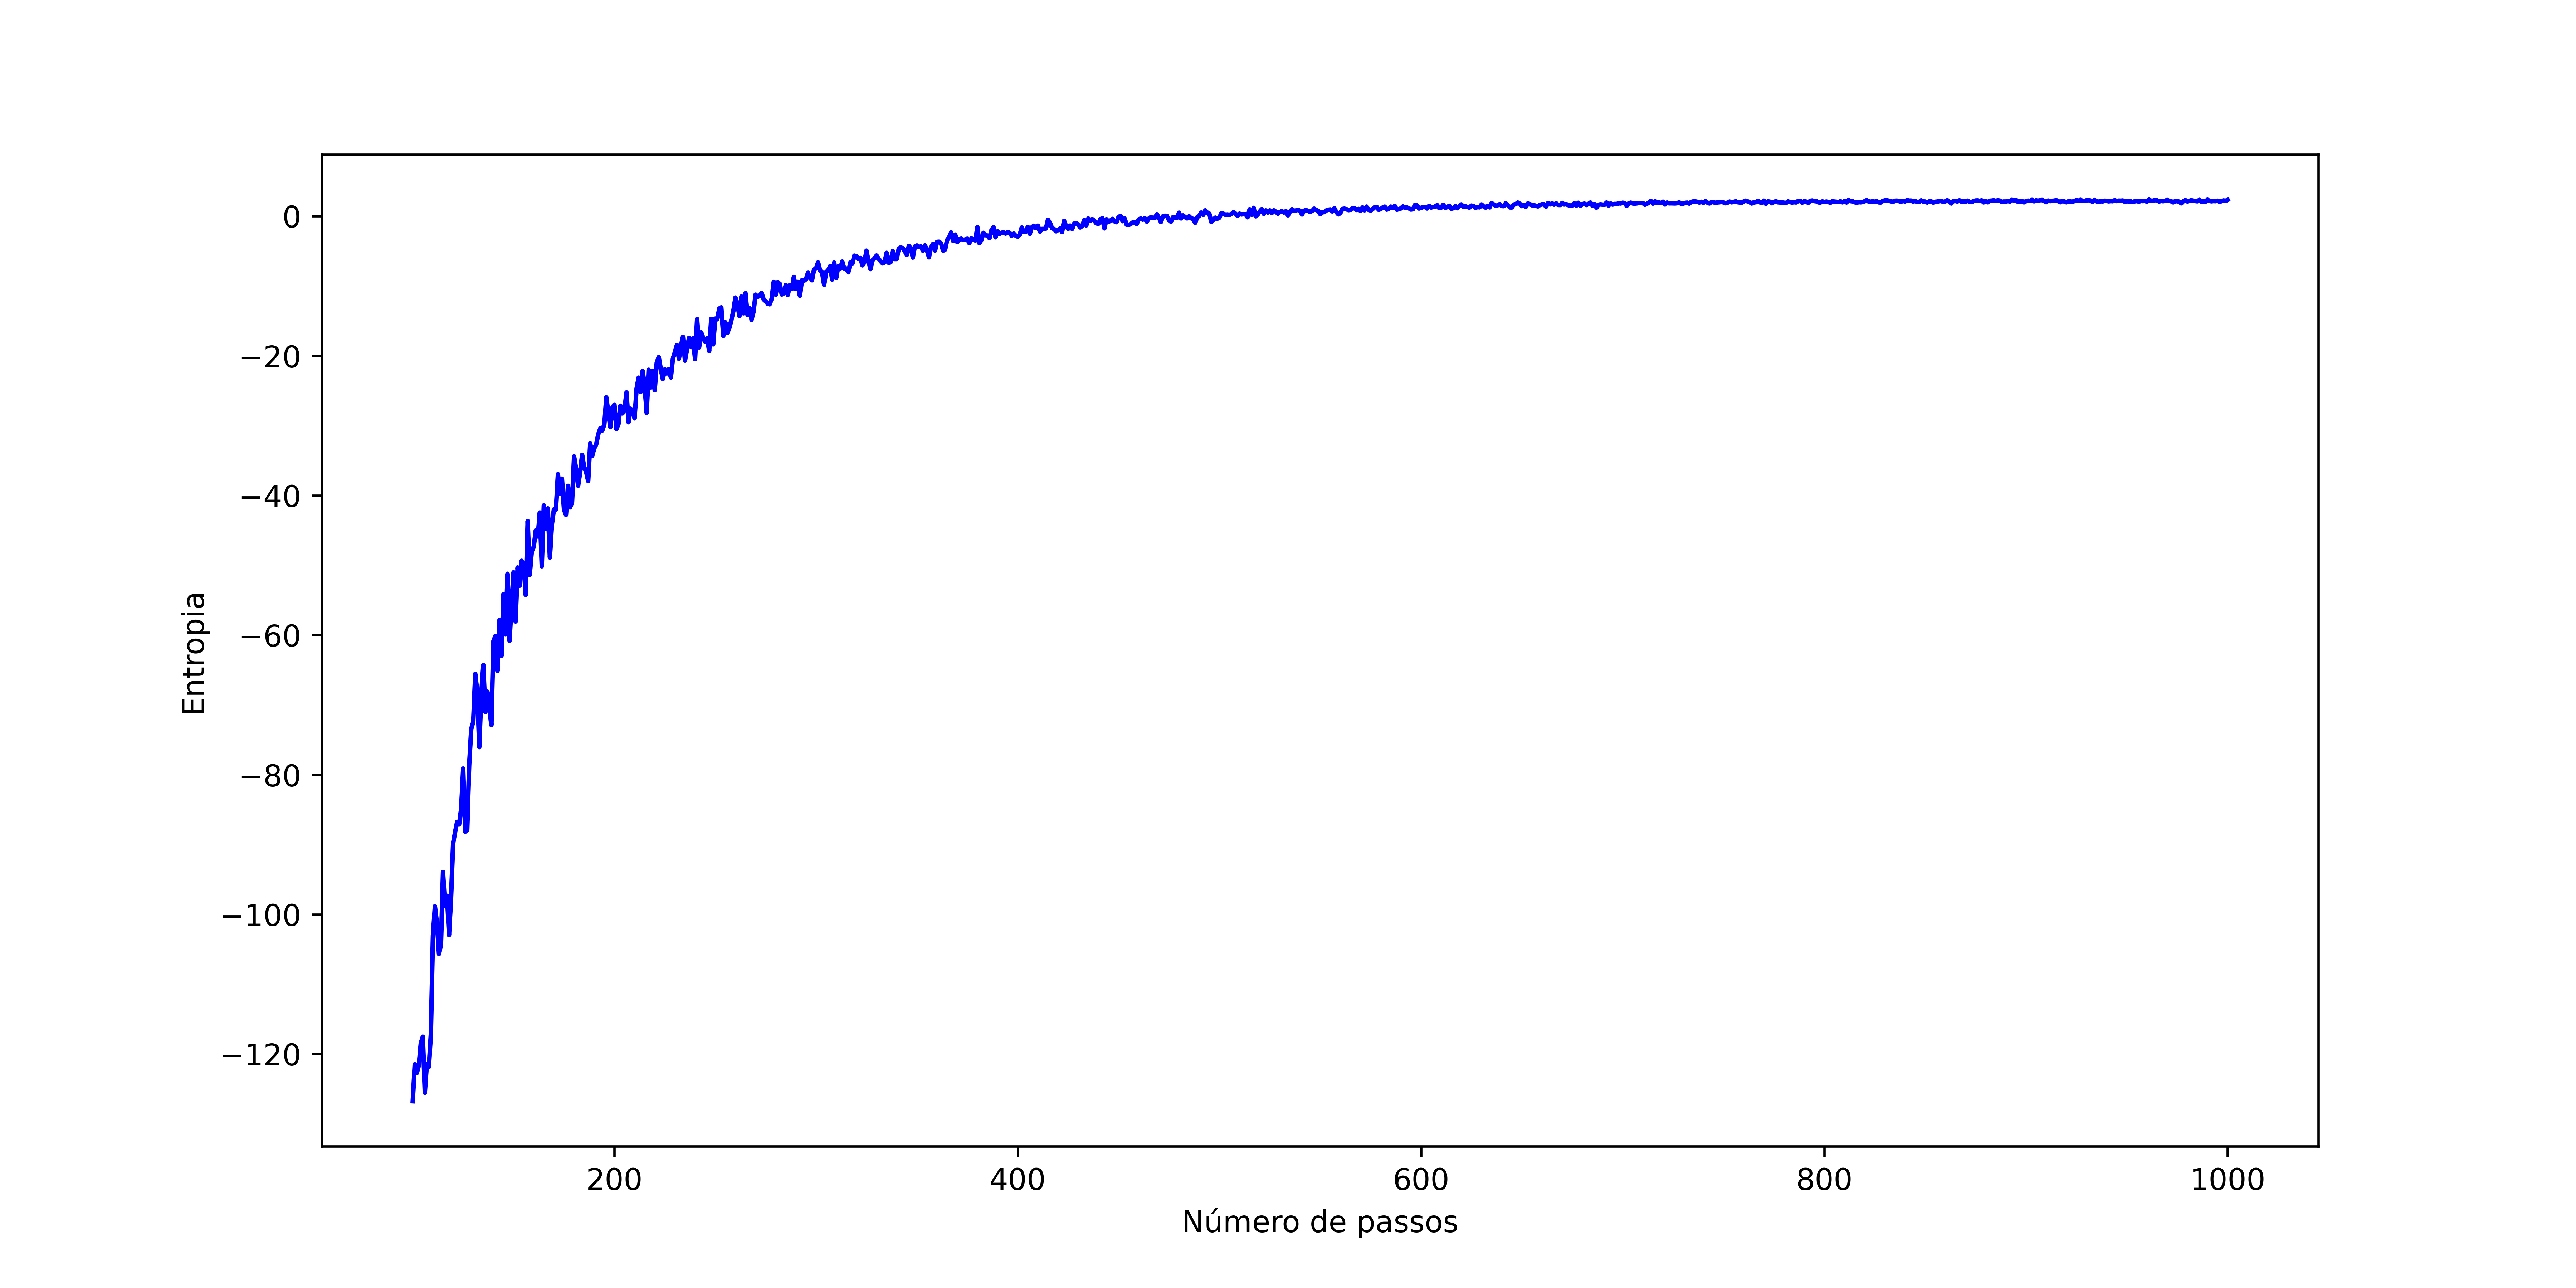
\includegraphics[width=16cm]{images/tarefa-4/tarefa-4-graf-1.png}
\caption{Entropia do sistema vs número de passos}

\caption*{Fonte: Compilado pelo Autor.}
\label{fig:tarefa 4 - Gráfico entropia versus número de passos}
\end{figure}
% ----------------------------------------------------------
% ELEMENTOS PÓS-TEXTUAIS
% ----------------------------------------------------------
% \bibliography{references}


%---------------------------------------------------------------------
% INDICE REMISSIVO
%---------------------------------------------------------------------
\printindex
%---------------------------------------------------------------------

\end{document}